\documentclass[11pt,a4paper]{article}
\usepackage[utf8]{inputenc}
\usepackage[T1]{fontenc}
\usepackage{lmodern}
\usepackage[margin=2.1cm]{geometry}
\usepackage{graphicx}
\usepackage{amsmath}
\usepackage{booktabs}
\usepackage{tabularx}
\usepackage{longtable}
\usepackage{array}
\usepackage{xcolor}
\usepackage{caption}
\usepackage{float}
\usepackage{enumitem}
\usepackage[colorlinks=true,linkcolor=blue!50!black,urlcolor=blue!60!black,citecolor=blue!50!black]{hyperref}
\usepackage{url}\def\UrlBreaks{\do\/\do-\do_\do.}

\setlist{itemsep=2pt,topsep=4pt}
\emergencystretch=3em
\captionsetup{font=small,labelfont=bf}
\DeclareUrlCommand\code{\urlstyle{tt}}
\newcommand{\codec}[1]{\texttt{\detokenize{#1}}}
\newcommand{\www}{https://vdamante.web.cern.ch/H_mumu/skim_v4}
\newcommand{\weblink}[2]{\href{\www/#1}{#2}}
\newcolumntype{Y}{>{\raggedright\arraybackslash}X}
\newcommand{\done}{\textcolor{green!45!black}{\textbf{done}}}
\newcommand{\miss}{\textcolor{red!70!black}{\textbf{missing}}}
\newcommand{\prog}{\textcolor{orange!85!black}{\textbf{in progress}}}
\newcommand{\inval}{\textcolor{red!70!black}{\textbf{done, invalid}}}

\title{The analysis DNN and the VBF selector\\[4pt]
\large $H\to\mu\mu$ Run~3 analysis (skim\_v4): purpose, training, architecture,\\
results and fit plan}
\author{Valeria D'Amante}
\date{7 October 2026}

\begin{document}
\maketitle

\begin{abstract}
\noindent
The Run~3 $H\to\mu\mu$ analysis uses two neural networks with different jobs.
\begin{itemize}
  \item The \textbf{analysis DNN} (\code{DNN_NNOutput}) separates the
  $H\to\mu\mu$ signal (VBF~H + ggH) from the background inside the cut-based VBF
  category. Its distribution is the fit variable of the \textsc{Combine}
  likelihood.
  \item The \textbf{VBF selector} (\code{VBFSel_NNOutput}) tags the
  \emph{VBF topology} (VBF~H + electroweak Z$jj$) against everything else, in all
  events with at least two jets. It does not use the dimuon mass. Its first use
  is to measure the EWK~Z normalisation in the dimuon-mass sidebands, which is
  the leading uncertainty of the DNN fit. It could later define an alternative
  VBF category.
\end{itemize}
This note covers, for both networks: the signal definition, training region and
sample, input features, architecture and training procedure, deployment in the
framework, and every result available on 7~October~2026. The last part lists
all fits, with and without systematic uncertainties, with and without the VBF
split by tag-jet pseudorapidity (CC/CF/FF). Each fit is marked done, invalid,
in progress or missing, and the planned order is given.
\end{abstract}

\tableofcontents
\newpage

%=====================================================================
\section{Analysis context}
%=====================================================================

\subsection{Event selection, categories and mass regions}
\paragraph{Baseline selection.}
\begin{itemize}
  \item Two opposite-sign muons, \code{HLT_IsoMu24} with trigger matching.
  \item $p_T(\mu_1) > 26$~GeV and $p_T(\mu_2) > 20$~GeV, $|\eta| < 2.4$.
  \item Medium ID, $|d_z| < 0.1$~cm, $|d_{xy}| < 0.05$~cm.
  \item Relative isolation with the FSR photon subtracted, below 0.25.
  \item Exactly two loose muons and no good electron.
  \item b-jet veto (UParT/PNet working points).
  \item The muon four-momentum includes the beam-spot constraint (bsc),
  scale and resolution corrections (ScaRe) and FSR recovery.
\end{itemize}

\paragraph{Jets.}
\begin{itemize}
  \item AK4, JEC and JER applied, tight ID, jet veto maps.
  \item Cleaned against the selected leptons.
  \item ``Horn'' veto against noisy forward jets:
  \begin{itemize}
    \item 2022--23: every jet with $|\eta| \ge 2.5$ and $p_T < 50$~GeV is removed;
    \item 2024--26: only jets with $2.5 \le |\eta| < 3.0$ and $p_T < 50$~GeV are
    removed.
  \end{itemize}
\end{itemize}

\paragraph{Categories.}
\begin{itemize}
  \item \textbf{VBF} (cut-based): a VBF jet pair with $p_T > 35/25$~GeV,
  $m_{jj} > 400$~GeV and $|\Delta\eta_{jj}| > 2.5$. The production pair is the
  one with the largest $m_{jj}$.
  \item \textbf{ggF}: baseline events that fail the VBF requirement. It has
  sub-categories by jet multiplicity (0J, 1J, 2J, $\ge$2J).
  \item \code{baseline_ge2J}: baseline with at least two jets, which equals
  \code{ggF_ge2J} + \code{VBF_ge2J}.
  \item \textbf{CC/CF/FF}: the VBF category split by the $|\eta|$ of the two tag
  jets, C if $|\eta| < 2.5$ and F if $|\eta| \ge 2.5$. ``incl'' is the unsplit
  category.
\end{itemize}

\begin{table}[H]\centering\small
\begin{tabular}{lll}
\toprule
region & $m_{\mu\mu}$ [GeV] & role \\
\midrule
Z sideband (ZSB) & 76--110 & control region; EWK~Z fit \\
H sideband (HSB) & 110--115 and 135--150 & control region in the $H\to\mu\mu$ fit; EWK~Z fit \\
Signal\_Fit (SR) & 115--135 & signal region (blinded above DNN $=0.8$) \\
Signal\_ext & 110--150 & plots \\
\bottomrule
\end{tabular}
\caption{Dimuon-mass regions.}
\end{table}

\paragraph{Eras and luminosity.} 2022, 2022EE, 2023, 2023BPix, 2024, 2025 and
2026: 308.8~fb$^{-1}$ in total, 283.0~fb$^{-1}$ for 2022--2025.

\paragraph{Plots.} All plots quoted here are under \url{\www/}, which is
\code{/eos/user/v/vdamante/www/H_mumu/skim_v4/}.

\subsection{Elements shared by the two networks}
\begin{itemize}
  \item \textbf{Network type.} Both are fully connected binary classifiers (MLP)
  with a sigmoid output.
  \item \textbf{k-fold.} Both use 4 folds.
  \begin{itemize}
    \item Model $k$ is trained without the events with
    \texttt{FullEventId~\%~4} $= k$.
    \item In the framework, each event is scored by model
    \texttt{FullEventId~\%~4}, so no event is ever scored by a model that saw it
    in training.
  \end{itemize}
  \item \textbf{ONNX.} The models are exported to ONNX with the input
  standardisation $(x-\mu)/\sigma$ inside the graph. Inference uses
  \code{onnxruntime} on CPU (\code{common/dnn_application.py}), and the
  histogram maker books the score for every variable ending in \code{_NNOutput}.
  \item \textbf{Systematic variations.}
  \begin{itemize}
    \item For the jet (JES, JER) and muon (scale/resolution) variations the
    score is \emph{re-evaluated} on the shifted inputs
    (\code{ApplyDNNVariations}), together with the derived observables
    (Zeppenfeld variable, $R_{p_T}$, soft activity, \dots).
    \item Before 29~September~2026 this was not the case: the score fell back
    to the nominal value, so jet and muon systematics only moved events
    across the selection. JES Absolute changes the DNN score of 16\% of the
    events and the VBF selector score of 52\%.
  \end{itemize}
\end{itemize}

%=====================================================================
\section{The analysis DNN (\texttt{DNN\_NNOutput})}
%=====================================================================

\subsection{Purpose and signal definition}
The DNN classifies events of the cut-based VBF category in the signal mass
window.
\begin{itemize}
  \item \textbf{Signal}: VBF~H (\code{VBFHto2Mu}) and ggH (\code{GluGluHto2Mu}),
  both with $m_H = 125$~GeV. The ggH events that pass the VBF selection are
  treated as signal, and the fit has a single signal strength $r$ for the
  sum.
  \item \textbf{Background}: everything else.
  \begin{itemize}
    \item Training: Drell--Yan ($m_{\ell\ell}$ 105--160~GeV), electroweak
    Z$jj$ ($m_{\ell\ell}$ 105--160~GeV, Herwig), $t\bar t$, VV.
    \item Evaluation and fit: also single top, $tW$, $t\bar tX$, VVV, W+jets,
    VH and $t\bar tH$.
  \end{itemize}
  \item \textbf{Fit}: the score, binned in 14 bins per era, is fitted in the SR
  and in the HSB of the VBF category. The HSB constrains the background
  normalisations and shapes.
\end{itemize}

\subsection{Payloads and provenance}

\begin{table}[H]\centering\small
\begin{tabularx}{\textwidth}{lYY}
\toprule
payload & directories & status \\
\midrule
\code{updated_DNN} (production) & \code{common/updated_DNN_configs}, \code{common/updated_DNN_models} & used in every era (default \code{model_set="updated"}) \\
legacy & \code{common/dnn_configs}, \code{common/dnn_models} (\code{_2024} for 2024--26) & \code{model_set="legacy"}, comparisons only \\
VBFNet (PR \#21) & \code{common/vbfnet_configs}, \code{common/vbfnet_models} & not usable: saturates, AUC 0.39--0.47 on skim\_v4 \\
\bottomrule
\end{tabularx}
\caption{DNN payloads known to \codec{common/dnn_application.py}.}
\end{table}

The production model was not trained in this repository. The config field
\code{results_dir} points to \code{/eos/user/a/ayeagle/H_mumu/results/OGDNN_big_run/}.
The description below is reconstructed from three sources: the deployed config,
the ONNX graph, and the training-tuple configuration kept in the repository
(\code{studies/dnn/traintuple_config_DNN.yaml}).

\subsection{Training region and sample}

\begin{table}[H]\centering\small
\begin{tabularx}{\textwidth}{lY}
\toprule
selection & \texttt{(Signal\_Fit) \& (VBF)}: cut-based VBF category, $115 < m_{\mu\mu} < 135$~GeV \\
processes & DY $m_{\ell\ell}$ 105--160, $t\bar t$, EWK~Z$jj$ 105--160 (Herwig), VV, VBF~H and ggH (amc@NLO) \\
eras & 2022--2025, distinguished by the input \code{era_code} (0 to 5); 2026 is evaluated with the 2025 code \\
labels & signal $=$ \code{VBFHto2Mu}, \code{GluGluHto2Mu}; everything else is background \\
weights & \code{weight__Central} in absolute value (\code{abs_train_weight = true}); signal and background sums equalised (\code{equalize_for_training}) \\
inputs & standardised with the training mean and standard deviation (\code{renorm_inputs}) \\
folds & $k = 4$; 33\% of the training folds used for validation \\
\bottomrule
\end{tabularx}
\caption{Training set-up of the production DNN.}
\end{table}

\subsection{Input features (32)}

\begin{longtable}{p{0.33\textwidth}p{0.6\textwidth}}
\toprule
feature & meaning \\
\midrule
\endhead
\code{era_code} & era index, 0 = 2022 \dots\ 5 = 2025 (2026 $\to$ 5) \\
\code{mu1_pt}, \code{mu1_eta}, \code{mu2_pt}, \code{mu2_eta} & leading and subleading muon kinematics \\
\code{m_mumu}, \code{pt_mumu}, \code{eta_mumu}, \code{phi_mumu}, \code{y_mumu} & dimuon system \\
\code{dR_mumu} & $\Delta R$ between the muons \\
\code{cosTheta_CS}, \code{phi_CS} & Collins--Soper angles \\
\code{R_pt} & $p_T$ balance of the dimuon + tag-jet system \\
\code{minDeltaEtaSigned}, \code{minDeltaPhi} & smallest $\Delta\eta$ and $\Delta\phi$ between the dimuon and a tag jet \\
\code{Zeppenfeld_Var} & dimuon rapidity relative to the tag jets, $(y_{\mu\mu} - \bar y_{jj})/|\Delta y_{jj}|$ \\
\code{pt_centrality} & $p_T$ centrality of the dimuon with respect to the tag jets \\
\texttt{vbfjet\{1,2\}\_pt}, \texttt{\_eta}, \texttt{\_y} & tag-jet kinematics \\
\texttt{vbfjet\{1,2\}\_btagPNetQvG} & quark/gluon discriminant of the tag jets \\
\code{m_jj}, \code{delta_eta_jj}, \code{pt_vbfj1j2} & dijet mass, $|\Delta\eta|$ and $p_T$ of the tag-jet pair \\
\code{N_SelectedJets} & jet multiplicity \\
\code{SoftJetCleanedActivity_N}, \code{_ptSum} & soft hadronic activity outside the tag jets and muons \\
\bottomrule
\caption{Inputs of the production DNN, in the payload order (32 features).}
\end{longtable}

$m_{\mu\mu}$ is an input, so the score can sculpt the mass distribution. The
fit uses the score in fixed mass regions, so this does not bias the fit, but
it ties the score shape to the mass resolution. The retraining
(\S\ref{sec:retraining}) has a second candidate without \code{m_mumu}.

\subsection{Architecture and training procedure}

\begin{table}[H]\centering\small
\begin{tabular}{ll}
\toprule
layers (from the ONNX graph) & $32 \to 86 \to 86 \to 86 \to 86 \to 1$ (Gemm) \\
activation & ReLU; sigmoid output \\
regularisation & none: \code{dropout = 0}, \code{batch_renorm = false} \\
loss & weighted binary cross-entropy \\
optimiser & Adam, learning rate $10^{-3}$, weight decay 0 \\
batch size & 10\,000 \\
epochs & \code{epochs = 1} in the deployed config, early stopping with patience 10 \\
trainable parameters & $32\cdot86 + 3\cdot86^2 + 86 + 5$ biases $\approx 2.5\times10^4$ \\
\bottomrule
\end{tabular}
\caption{Production DNN (\codec{common/updated_DNN_configs/config.toml}).}
\end{table}

The deployed config sets one epoch. The retraining config of 30~September
sets 200 epochs with early stopping, to correct the training length.

\paragraph{Legacy payload.}
\begin{itemize}
  \item 26 inputs: the same as above without \code{era_code}, the tag-jet
  rapidities, \code{pt_vbfj1j2}, \code{N_SelectedJets} and the soft activity, and
  with \code{pt_jj}.
  \item ONNX graph $26 \to 50 \to 50 \to 50 \to 50 \to 1$. The config says
  \code{[52, 26, 26, 13]}; the graph is authoritative.
  \item Trained on \texttt{VBF\_JetVeto \& Signal\_Fit}, with Adam (lr $10^{-4}$),
  batch 1200, 64 epochs and patience 20.
\end{itemize}

\subsection{Deployment and templates}
\begin{itemize}
  \item \textbf{Score.} \code{DNN_NNOutput} is computed in
  \code{histograms/hist_maker.py} for the nominal and for every jet/muon
  variation.
  \item \textbf{Fit binning.} 14 bins per era (\code{config/plot/histograms.yaml});
  the SR is split at DNN $=0.8$ for blinding.
  \item \textbf{Histogram campaigns:}
  \begin{itemize}
    \item \code{dnn_vbf}: VBF category, five mass regions, all systematic
    families, DY/EWK jet components. Used for the plots.
    \item \code{dnn_vbf_eta_regions_syst}: the same with the CC/CF/FF split;
    the \code{incl} sub-directory is the unsplit category. These are
    \emph{the fit templates from now on}, both inclusive and split.
    \item \code{dnn_vbf_eta_regions}: CC/CF/FF, Central only. It was used for
    the categorisation study.
    \item \code{dnn_vbf_weighted} (17~September): produced before the score
    was re-evaluated for jet and muon variations, so its JES/JER/muon-scale
    templates are wrong. Every DNN fit with systematics quoted below used it.
  \end{itemize}
  \item \textbf{DY reweighting.} DY carries three reweightings: jet component,
  $p_T(\ell\ell)$ and $N_\text{jets}$. DY is split into \emph{Hard} and
  \emph{PU1}/\emph{PU2} components, according to whether the tag jets match
  generator jets or come from pile-up.
\end{itemize}

\subsection{Results: separation power}

\begin{table}[H]\centering\small
\begin{tabular}{lcccccc|c}
\toprule
era & 2022 & 2022EE & 2023 & 2023BPix & 2024 & 2025 & 2026$^\ast$ \\
\midrule
weighted AUC & 0.905 & 0.903 & 0.908 & 0.899 & 0.890 & 0.888 & 0.905 \\
$S$ (events) & 1.8 & 6.0 & 4.0 & 2.2 & 43.3 & 45.2 & -- \\
$B$ (events) & 382 & 1153 & 923 & 498 & 9267 & 9323 & -- \\
best cut & 0.921 & 0.919 & 0.920 & 0.950 & 0.944 & 0.871 & -- \\
best $S/\sqrt{S+B}$ & 0.287 & 0.491 & 0.375 & 0.275 & 1.113 & 1.086 & -- \\
signal eff.\ at best cut & 0.44 & 0.44 & 0.45 & 0.30 & 0.24 & 0.40 & -- \\
\bottomrule
\end{tabular}
\caption{\codec{DNN_NNOutput} in \codec{Signal_Fit_VBF}, from the histograms with the DY
weights (\codec{results/skim_v4/dnn_performance/dy_weights_weighted/}).
$^\ast$2026: ROC from the skims, 30 files per dataset (\codec{roc_from_skims}).
The DY weights change the AUC by $-0.005$ (2024) and the best $S/\sqrt{S+B}$ by $+2.5\%$.}
\end{table}

\begin{figure}[H]\centering
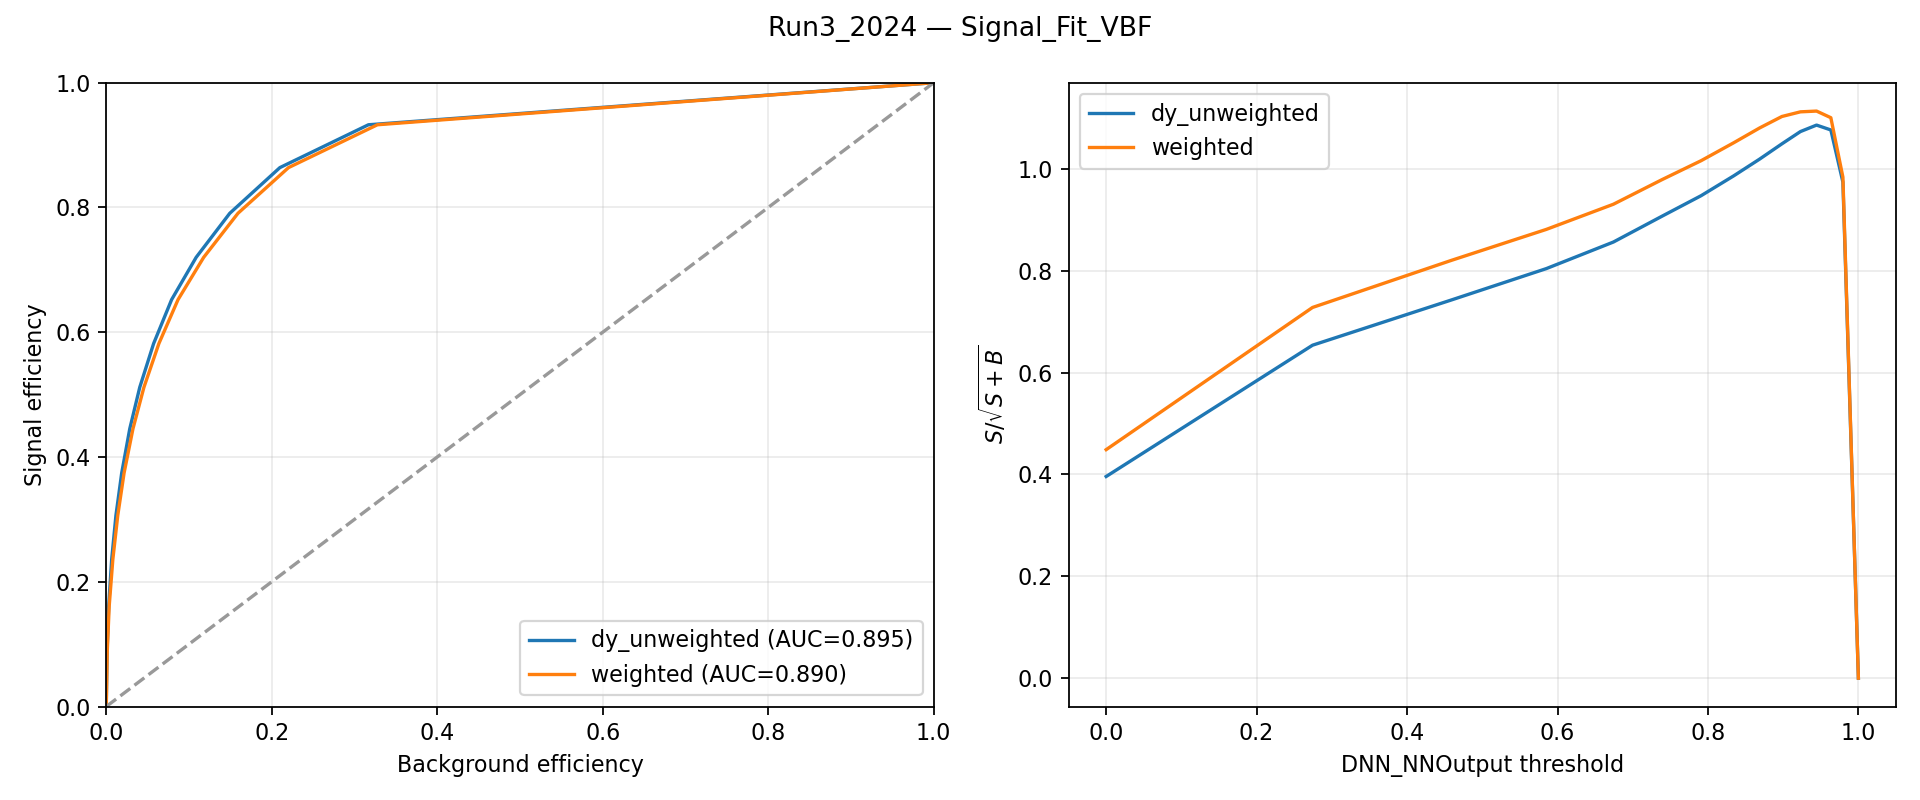
\includegraphics[width=0.85\textwidth]{figures/dnn_roc_2024.png}
\caption{DNN, 2024, SR of the VBF category: ROC curve and $S/\sqrt{S+B}$ as a
function of the threshold, with and without the DY weights.
\weblink{studies/dnn/dnn_performance/}{All eras}.}
\end{figure}

\subsection{Results: binning of the score}
\code{studies/dnn/optimize_dnn_binning.py} scans contiguous partitions that
maximise the binned Asimov significance. It uses statistics only and requires
at least 10 background events per bin.

\begin{table}[H]\centering\small
\begin{tabular}{lcccccc}
\toprule
& 2022 & 2022EE & 2023 & 2023BPix & 2024 & 2025 \\
\midrule
best single cut & 0.276 & 0.507 & 0.385 & 0.267 & 1.171 & 1.114 \\
5 bins & 0.292 & 0.575 & 0.438 & 0.289 & 1.540 & 1.493 \\
gain & +6\% & +13.5\% & +13.7\% & +8.4\% & +31.5\% & +34\% \\
\bottomrule
\end{tabular}
\caption{Binned Asimov significance, statistics only.}
\end{table}

Five bins recover 98--99.8\% of the maximum, and the last bin sits on the
10-event floor, so the MC statistics sets the edges. The fit uses 14 bins;
\code{autoMCStats} costs about $0.08\,\sigma$. 2026 is not in this scan.

\begin{figure}[H]\centering
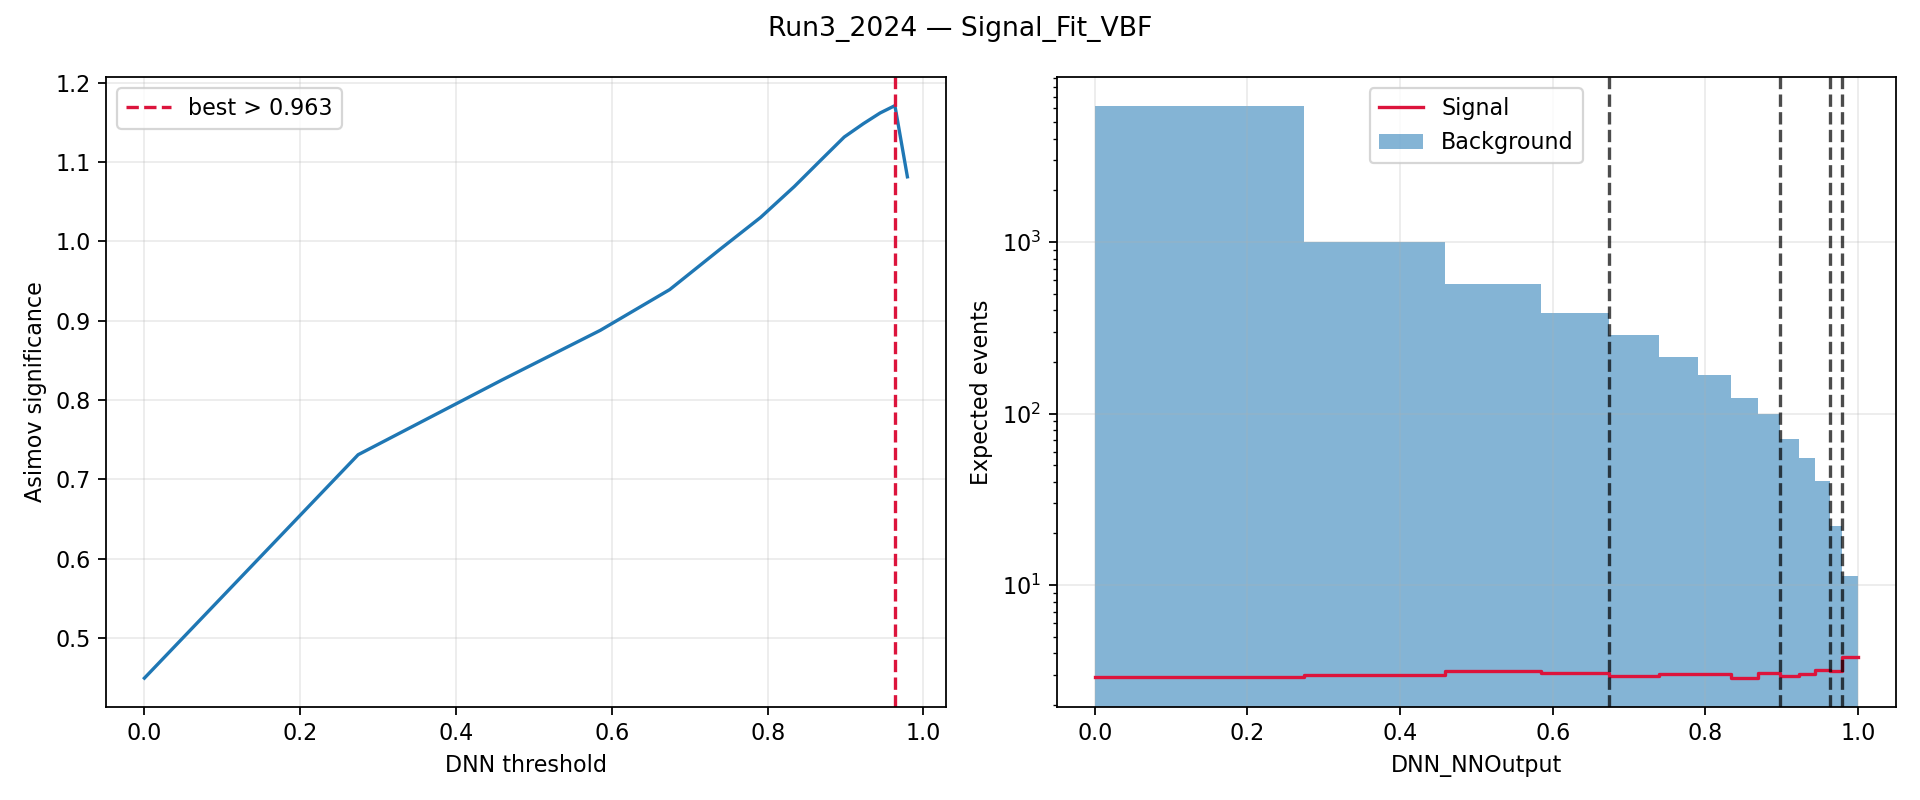
\includegraphics[width=0.62\textwidth]{figures/dnn_binning_2024.png}\hfill
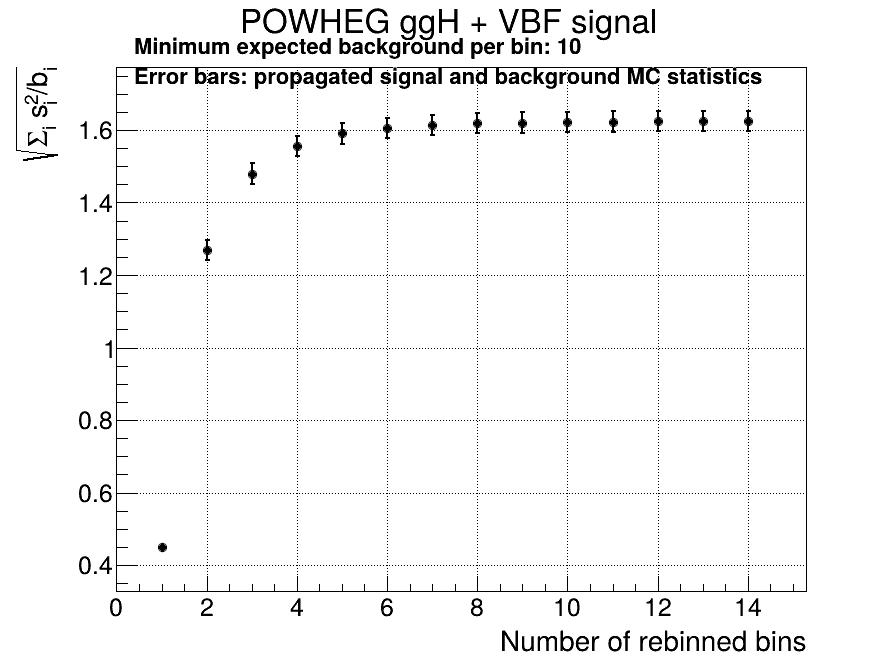
\includegraphics[width=0.36\textwidth]{figures/dnn_sensitivity_2024.png}
\caption{Left: Asimov significance against the DNN threshold and optimised
edges, 2024. Right: $\sqrt{\sum_i s_i^2/b_i}$ against the number of bins, 2024,
POWHEG signal.
Links: \weblink{studies/dnn/dnn_binning/}{binning} and
\weblink{studies/dnn/sensitivity/}{sensitivity}.}
\end{figure}

\subsection{Results: data/MC}
Figure~\ref{fig:dnn-dmc} shows the score in the HSB of the VBF category, with
the Hard/PU composition of every process. The SR is blinded above DNN $=0.8$.
At high score the forward-forward tag-jet configuration (FF) has the worst
data/MC: $+18\%$ in 2024 and $+30\%$ in 2025 for DNN $> 0.94$. All eras and
regions are in \weblink{dnn/data_mc/}{dnn/data\_mc}, and the systematic shapes
in \weblink{dnn/systematics/}{dnn/systematics}.

\begin{figure}[H]\centering
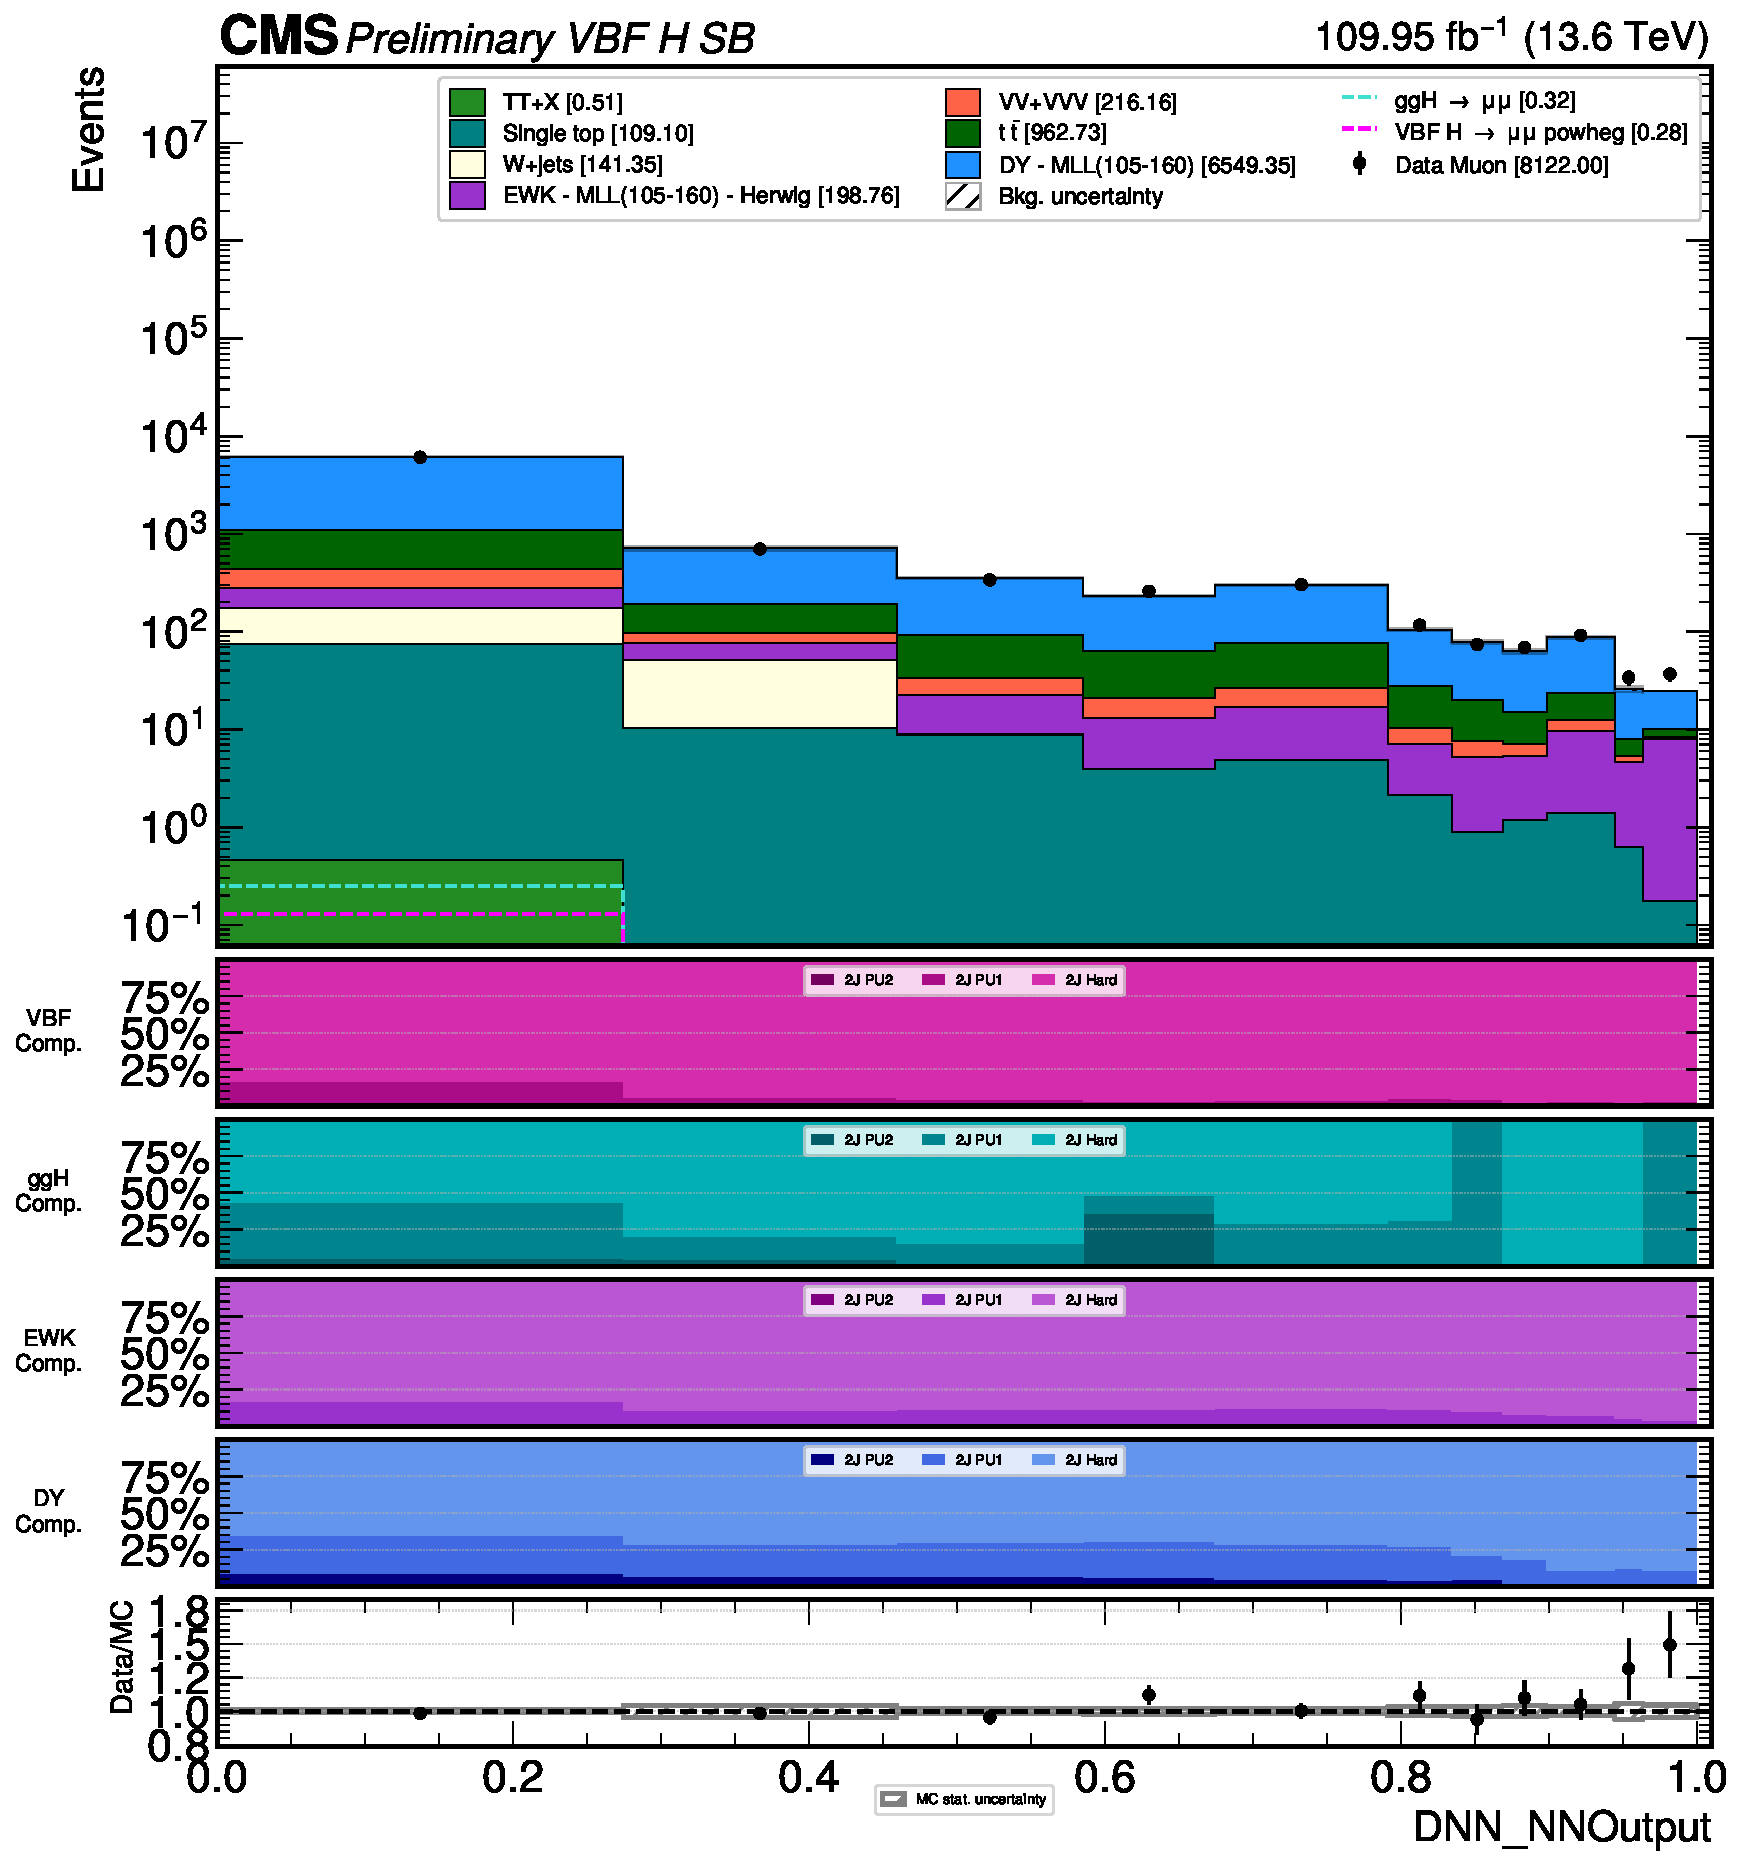
\includegraphics[width=0.55\textwidth]{figures/dnn_datamc_hsb_2024.pdf}
\caption{\codec{DNN_NNOutput} in the HSB of the VBF category, 2024, with the Hard/PU
composition of VBF~H, ggH, EWK~Z and DY.}
\label{fig:dnn-dmc}
\end{figure}

\subsection{\textsc{Combine} fit set-up}
\begin{itemize}
  \item \textbf{Channels:} \code{Signal_Fit_VBF} and \code{H_sideband_VBF}, one
  pair per era. Each era has 14 bins, and the SR is split at DNN $=0.8$.
  \item \textbf{Signal:} VBF~H + ggH with a single POI $r$ and
  \code{--expectSignal 1}.
  \item \textbf{Systematics:}
  \begin{itemize}
    \item shape: JER in 6 $\eta/p_T$ bins, JES as 11 regrouped sources (or
    the total), muon efficiencies, muon scale and resolution (ScaRe), PDF,
    pile-up, QCD scales, and the parton shower for EWK~Z and VBF~H;
    \item normalisation: luminosity and cross-section lnN, built per source
    and weighted by the dataset yields;
    \item MC statistics through \code{autoMCStats} (Barlow--Beeston lite).
  \end{itemize}
  \item \textbf{DY models} (\code{--dy-model}):
  \begin{itemize}
    \item \code{lnn}: Hard, PU1 and PU2 with an lnN from the error of the
    0/1/2-jet fit;
    \item \code{rateparam-pu}: PU1+PU2 free, Hard lnN;
    \item \code{rateparam-both}: Hard and PU free;
    \item \code{inclusive}: one free DY template.
  \end{itemize}
  \item \textbf{Asimov datasets:}
  \begin{itemize}
    \item \emph{pre-fit}: nuisances at their nominal values;
    \item \emph{toysFreq} (the reference): the nuisances are first fitted to
    the data with $r = 1$, with the SR above DNN $=0.8$ masked, and the Asimov is
    then generated from that point.
  \end{itemize}
  The old one-line \code{--toysFreq} also fitted the high-score SR data and is
  no longer used.
  \item \textbf{Stat-only:} \code{--freezeParameters allConstrainedNuisances};
  free rateParams stay free.
  \item \textbf{Tools:} \code{combine/build_signal_extended_datacards.py},
  \code{combine/fit_suite.py} and \code{combine/run_fit_matrix.sh} (every era and
  all eras).
\end{itemize}

\subsection{Results: expected significance}
These results are the fit matrix of 4~October~2026, with seven eras. They used
the old \code{dnn_vbf_weighted} templates (see the caveats).

\begin{table}[H]\centering\small
\begin{tabular}{lccccc}
\toprule
DY model & SR, pre-fit & SR, toysFreq & SR+HSB, pre-fit & SR+HSB, toysFreq & $r$, SR+HSB, toysFreq \\
\midrule
\code{lnn} & 1.964 & 1.932 & 2.135 & \textbf{2.102} & $1.00^{+0.50}_{-0.48}$ \\
\code{rateparam-pu} & 1.933 & 1.874 & 2.090 & 2.019 & $1.00^{+0.53}_{-0.50}$ \\
\code{rateparam-both} & 1.650 & 1.619 & 1.991 & 1.876 & $1.00^{+0.55}_{-0.54}$ \\
\code{inclusive} & 1.844 & 1.744 & 2.029 & 1.879 & $1.00^{+0.55}_{-0.54}$ \\
\bottomrule
\end{tabular}
\caption{Expected significance ($\sigma$), full systematics, seven eras.
Stat only (\codec{lnn}, SR+HSB, toysFreq): 2.476, with
$r = 1.00^{+0.43}_{-0.42}$. Median expected limits (pre-fit, 30~September):
0.918 (\codec{lnn}), 0.938 (\codec{rateparam-pu}), 0.988 (\codec{rateparam-both}).}
\end{table}

\begin{table}[H]\centering\small
\begin{tabular}{lcccc}
\toprule
era & SR+HSB pre-fit & SR+HSB toysFreq & toysFreq stat only & SR only pre-fit / toysFreq \\
\midrule
2022 & 0.326 & 0.323 & 0.365 & 0.325 / 0.323 \\
2022EE & 0.578 & 0.564 & 0.640 & 0.567 / 0.544 \\
2023 & 0.406 & 0.409 & 0.488 & 0.405 / 0.408 \\
2023BPix & 0.323 & 0.318 & 0.363 & 0.320 / 0.311 \\
2024 & 1.365 & 1.313 & 1.524 & 1.266 / 1.259 \\
2025 & 1.288 & 1.284 & 1.513 & 1.132 / 1.124 \\
2026 & 0.707 & 0.711 & 0.783 & 0.693 / 0.704 \\
all & 2.135 & 2.102 & 2.476 & 1.964 / 1.932 \\
\bottomrule
\end{tabular}
\caption{Per era, \codec{lnn}.}
\end{table}

\begin{itemize}
  \item \textbf{toysFreq vs pre-fit.} toysFreq is 1.5\% (\code{lnn}) to 7.4\%
  (\code{inclusive}) lower than the pre-fit Asimov. The data pull the nuisances
  in the direction that reduces the sensitivity, more where DY is freer.
  \item \textbf{HSB.} It adds 8.8\% (\code{lnn}) and 15.9\% (\code{rateparam-both}).
  \item \textbf{Leading impacts} (\code{lnn}, SR+HSB, toysFreq):
  \begin{itemize}
    \item \code{QCD_fac_scale_V} 0.127, mostly from EWK~Z at high score;
    \item JES Absolute 0.058 and RelativeBal 0.054, which are not reliable
    with the old templates;
    \item MC statistics of the last SR bins 0.050;
    \item \code{JEReta3pt02025} 0.048.
  \end{itemize}
  \item \textbf{Statistics dominates.} Removing all constrained nuisances only
  reaches 2.51.
  \item \textbf{Pulls} of the toysFreq data fit: none beyond $1.8\sigma$.
  \item \textbf{Six eras.} Until 30~September, without 2026: 2.006 pre-fit
  (\code{lnn}, SR+HSB). The 2.23 of 2~September was inflated by a missing
  VBF-filtered DY sample in 2024--25.
\end{itemize}

\paragraph{EWK~Z normalisation.} At high score EWK~Z is 19--36\% of the
background and about 1.6 times the signal. In the cards it is constrained only
by the $\pm0.5\%$ generator integration error.

\begin{table}[H]\centering\small
\begin{tabular}{lcccc}
\toprule
EWK~Z normalisation & $\pm0.5\%$ & lnN 10\% & lnN 30\% & free \\
\midrule
expected $Z$ & 2.14 & 2.07 & 1.86 & 1.63 ($-23\%$) \\
\bottomrule
\end{tabular}
\caption{Dependence of the DNN fit on the EWK~Z normalisation
(\codec{docs/ewkz_fit_motivation.md}, \codec{results_fit_matrix/dnn_ewk_norm_test}).}
\end{table}

The DNN separates H from the background, but it does not separate EWK~Z from
DY. This is the motivation for the VBF selector (\S\ref{sec:vbfsel}).

\subsection{Studies built on the DNN}
\paragraph{VBF split by tag-jet $\eta$ (CC/CF/FF).}
\begin{itemize}
  \item \textbf{Cards:} \code{studies/sensitivity_levers/central_cards.py}.
  \begin{itemize}
    \item Central templates of \code{dnn_vbf_eta_regions}.
    \item DY reweighted but not split into Hard/PU.
    \item Only data statistics, MC statistics and luminosity.
  \end{itemize}
  \item \textbf{Result:} only the ratio split/incl is meaningful.
\end{itemize}

\begin{table}[H]\centering\small
\begin{tabular}{llccc}
\toprule
eras & Asimov & incl & CC/CF/FF & gain \\
\midrule
6 & one-line \code{--toysFreq} (SR in the data fit) & 2.255 & 2.429 & +7.7\% (artefact) \\
6 & pre-fit & 2.236 & 2.278 & +1.9\% \\
6 & pre-fit, free DY per era and $\eta$ category & 2.225 & 2.267 & +1.9\% \\
7 & pre-fit & 2.350 & 2.393 & +1.8\% \\
7 & \textbf{toysFreq, whole SR masked} & 2.366 & 2.410 & \textbf{+1.8\%} \\
2026 & pre-fit & 0.726 & 0.732 & +0.8\% \\
\bottomrule
\end{tabular}
\caption{Expected significance, inclusive VBF against CC/CF/FF, no shape systematics.}
\end{table}

\begin{itemize}
  \item The +7.7\% quoted until 30~September came from fitting the
  MC-statistics parameters to the high-score FF data, which have an excess.
  \item The statistics-only binned estimate on 2022--2025 was +4.3\%.
\end{itemize}

\paragraph{Definition of the VBF jet pair.} Three definitions were compared: max
$m_{jj}$ (production), hardest, and two leading.

\begin{table}[H]\centering\small
\begin{tabular}{lccc}
\toprule
all eras, 308.8~fb$^{-1}$ & max $m_{jj}$ & hardest & two leading \\
\midrule
correct pair in VBF signal & 0.82 & 0.87 & \textbf{0.93} \\
VBF signal pair with $\ge1$ pile-up jet & 0.086 & 0.058 & \textbf{0.034} \\
$S/(S+B)$, SR, DNN $>0.8$ & 0.043 & 0.044 & \textbf{0.051} \\
signal kept & 100\% & 100\% & 79\% \\
Combine, production DNN, \code{lnn} & 1.976 & 2.021 & \textbf{2.064} \\
small DNN per definition (2024), \code{lnn} & 1.440 $\pm$ 0.018 & 1.373 $\pm$ 0.062 & 1.414 $\pm$ 0.047 \\
\bottomrule
\end{tabular}
\caption{VBF pair definitions. The small DNN is an MLP 64--32 on the 31
production inputs, retrained for each definition, with 2 folds on the event
parity and three seeds.}
\end{table}

With a dedicated network the three definitions have the same sensitivity
within the spread between seeds. The production pair is kept.

\paragraph{Horn veto in 2025--26.} The veto is needed in both eras: without
it, the $2.5<|\eta|<3.0$ window is the worst-modelled part of the jet $\eta$
spectrum. It moves 11\% of VBF~H from VBF to ggF and costs at most 2\% in the
VBF category.

\subsection{Retraining on seven eras}\label{sec:retraining}
\begin{itemize}
  \item \textbf{Status.} The config is ready in \code{studies/dnn/retraining/}
  (30~September) but the network has not been trained.
  \item \textbf{Set-up:}
  \begin{itemize}
    \item the same 32 features and architecture;
    \item \code{era_code} $=6$ for 2026;
    \item 4 folds on \texttt{FullEventId~\%~4};
    \item 200 epochs with early stopping (patience 10);
    \item output in \code{/eos/user/v/vdamante/H_mumu/skim_v4/dnn_retraining/run3_all_eras_20260930}.
  \end{itemize}
  \item \textbf{Comparisons:}
  \begin{enumerate}
    \item the same features, to isolate the effect of 2026 and of the training
    length;
    \item without \code{m_mumu}, to test mass sculpting.
  \end{enumerate}
  \item \textbf{Replacement rule.} The production payload is replaced only after
  a comparison with the same campaign, full systematics and the same card.
\end{itemize}

%=====================================================================
\section{The VBF selector (\texttt{VBFSel\_NNOutput})}\label{sec:vbfsel}
%=====================================================================

\subsection{Purpose and signal definition}
\begin{itemize}
  \item \textbf{What it is.} A binary classifier of the VBF topology.
  \begin{itemize}
    \item Signal: VBF~H (\code{VBFHto2Mu}) + EWK~Z$jj$ (\code{EWK}).
    \item Background: DY, ggH, $t\bar t$, VV.
  \end{itemize}
  \item \textbf{No dimuon mass.} The mass is not an input, so the score has the
  same meaning in the sidebands and in the SR.
  \item \textbf{What ``signal'' means in each region.} In the sidebands the VBF
  signal is almost entirely EWK~Z: in the 2024 HSB there are 0.6 VBF~H + ggH
  events against 199 EWK~Z. In the SR, VBF~H is a small fraction of the VBF
  signal.
  \item \textbf{Measurement.} Fitting the score in the Z and H sidebands
  therefore measures the EWK~Z signal strength $r_\text{EWK}$, and DY Hard/PU
  at the same time. EWK~Z behaves like a standard candle of the VBF topology,
  and its normalisation is the leading nuisance of the $H\to\mu\mu$ fit.
\end{itemize}

\paragraph{Uses.}
\begin{enumerate}
  \item EWK~Z normalisation in the sidebands, propagated to the $H\to\mu\mu$
  card as a constraint on EWK~Z (today it is constrained only at $\pm0.5\%$).
  \item A \emph{selector-defined VBF category} (score $>$ cut) replacing the
  cut-based one. This is still open.
  \item Validation, era by era, of the modelling of the tag-jet kinematics and
  of pile-up jets: a data/MC test of the VBF topology independent of the dimuon
  mass.
\end{enumerate}
The current $H\to\mu\mu$ pipeline still uses the cut-based VBF category.

\subsection{Training sample}

\begin{table}[H]\centering\small
\begin{tabularx}{\textwidth}{lY}
\toprule
selection & \texttt{baseline \&\& leadingjet\_pt \textgreater{} 0 \&\& subleadingjet\_pt \textgreater{} 0}, i.e.\ \code{baseline_ge2J} \\
models & \code{sidebands_only}: ZSB + HSB, background cap $3\times10^6$ \\
& \code{inclusive_regions}: ZSB + HSB + SR, cap $1.5\times10^6$; \textbf{deployed} since 29~September \\
signal samples & VBF~H powheg; EWK~Z$jj$: inclusive (\code{EWK_2L2J_madgraph_herwig}) in the ZSB, $m_{\ell\ell}$ 105--160 (Herwig) in the HSB and SR \\
background samples & DY M-50 (ZSB), DY 105--160 (+ \code{_Fil_VBF} in 2024--26) in the HSB and SR, ggH, $t\bar t$ (2L2$\nu$, 4Q, L$\nu$2Q), WW/WZ/ZZ. No single top, W or VVV \\
eras & all seven (2022--2026), skim\_v4; no era input \\
event weight & \code{weight__Central} with its sign (\code{abs_train_weight = false}) \\
class balance & signal sum $=$ background sum (\code{equalize_for_training}) \\
cap & per background (process, region, era); random subsample (seed 12345) reweighted by $N/N_\text{cap}$, so yields are unchanged; VBF~H and EWK~Z never subsampled \\
folds & $k=4$, test fold \texttt{FullEventId~\%~4}; the rest split 68/32 train/validation, stratified by process \\
\bottomrule
\end{tabularx}
\caption{Training sample of the VBF selector (\codec{studies/vbf_selector/}).}
\end{table}

\paragraph{Pipeline.}
\begin{enumerate}
  \item \code{make_training_tuples.py}: flat tuples per era and dataset from the
  skims, with sample routing to the regions.
  \item \code{build_train_sample.py}: capping and the single pickle
  (\code{train_sample_zhsr.pkl}, 8.1~GB).
  \item \code{model_train/}: training on GPU (\code{main_condor.py}), one job per
  fold, and ONNX export.
  \item \code{evaluate.py}: AUC per era and region, plus the cut scan.
  \item \code{shap_per_era.py}: SHAP values.
\end{enumerate}

\subsection{Input features (24)}
\begin{itemize}
  \item \code{pt_mumu}, the only dimuon quantity;
  \item \code{N_SelectedJets};
  \item for each of the four leading jets (\code{leadingjet}, \code{subleadingjet},
  \code{thirdjet}, \code{fourthjet}): $p_T$, $\eta$, $\phi$, \code{btagPNetQvG}
  (quark/gluon), \code{btagPNetCvL} (charm/light). Missing jets get a default
  value;
  \item \code{SoftJetCleanedActivity_N} and \code{SoftJetCleanedActivity_ptSum}.
\end{itemize}
The inputs and the network come from the VBFNet of PR~\#21 (A.~Yeagle). What
changed is the training region, the training length (one epoch in the PR) and
a dropout bug fix: in the PR the dropout stayed active in evaluation mode.

\subsection{Architecture and training procedure}

\begin{table}[H]\centering\small
\begin{tabular}{ll}
\toprule
layers & $24 \to 100 \to 100 \to 100 \to 100 \to 50 \to 50 \to 1$ \\
hidden block & Linear $\to$ BatchNorm1d $\to$ ReLU $\to$ Dropout($p=0.10$) \\
output & sigmoid; the network runs in float64 \\
loss & per-event BCE $\times$ training weight, averaged \\
optimiser & Adam, learning rate $5\times10^{-3}$, weight decay 0 \\
batch size & 10\,000, shuffled \\
duration & early stopping on the validation loss (patience 10), best state restored \\
standardisation & weighted mean and std.\ of the training split, embedded in ONNX \\
\bottomrule
\end{tabular}
\caption{VBF selector (\codec{common/vbfsel_configs/config.toml}). The config
sets a 200-epoch limit, but the early-stopping loop does not apply it.}
\end{table}

\paragraph{Deployment.}
\begin{itemize}
  \item Models: \texttt{common/vbfsel\_models/trained\_model\_\{0..3\}.onnx},
  byte-identical to \code{results_zhsr/fold_k}.
  \item Loss curves:
  \code{/eos/user/v/vdamante/H_mumu/skim_v4/vbf_selector/results_zhsr/fold_<k>/<k>_loss.svg}.
  \item The folds were trained on 29~September between 13:17 and 15:08.
  \item In the framework, NaN or infinite inputs are set to $-10^4$ and a NaN
  score to 0.
  \item Fit binning: edges at 0, 0.1, \dots, 0.8, 0.85, 0.9, 0.93, 0.95, 0.97,
  0.98, 0.99, 1.
\end{itemize}

\paragraph{Histogram campaigns.}
\begin{itemize}
  \item \code{vbf_selector_ewkz}:
  \begin{itemize}
    \item score and the 24 inputs, in the ZSB and HSB;
    \item categories \code{baseline_ge2J}, \code{ggF_ge2J}, \code{VBF_ge2J},
    \code{ggF} and \code{VBF};
    \item all systematics, DY/EWK jet components.
  \end{itemize}
  \item \code{vbf_selector_ewkz_eta}: the same in the VBF category split
  incl/CC/CF/FF.
\end{itemize}

\subsection{Results: separation power}

\begin{table}[H]\centering\small
\begin{tabular}{lccc|ccc}
\toprule
& \multicolumn{3}{c|}{\code{inclusive_regions}} & \multicolumn{3}{c}{\code{sidebands_only}} \\
region & all & VBF~H only & EWK~Z only & all & VBF~H only & EWK~Z only \\
\midrule
Z sideband & 0.8995 & 0.8281 & 0.8995 & 0.8998 & 0.8184 & 0.8998 \\
H sideband & 0.8237 & 0.8309 & 0.8237 & 0.8180 & 0.8224 & 0.8180 \\
Signal\_Fit & 0.8217 & 0.8447 & 0.8200 & 0.8157 & 0.8372 & 0.8141 \\
\bottomrule
\end{tabular}
\caption{Weighted ROC AUC, all eras, each event scored by the fold that did not
see it. \codec{sidebands_only} never saw the SR; adding the SR to the training
gains about 0.006.}
\end{table}

\begin{table}[H]\centering\small
\begin{tabular}{lccccccc}
\toprule
& 2022 & 2022EE & 2023 & 2023BPix & 2024 & 2025 & 2026 \\
\midrule
Z sideband & 0.900 & 0.900 & 0.902 & 0.902 & 0.900 & 0.897 & 0.904 \\
H sideband & 0.859 & 0.856 & 0.857 & 0.862 & 0.823 & 0.812 & 0.821 \\
Signal\_Fit & 0.853 & 0.854 & 0.851 & 0.856 & 0.821 & 0.811 & 0.819 \\
\bottomrule
\end{tabular}
\caption{AUC per era (\codec{inclusive_regions}).}
\end{table}

The drop from about 0.855 (2022--23) to about 0.815 (2024--26) follows the
change of the horn veto. In 2024--26 it covers only $2.5 \le |\eta| < 3.0$, and
58--63\% of the VBF-category DY has a pile-up tag jet, against 16--21\% in
2022--23.

\begin{figure}[H]\centering
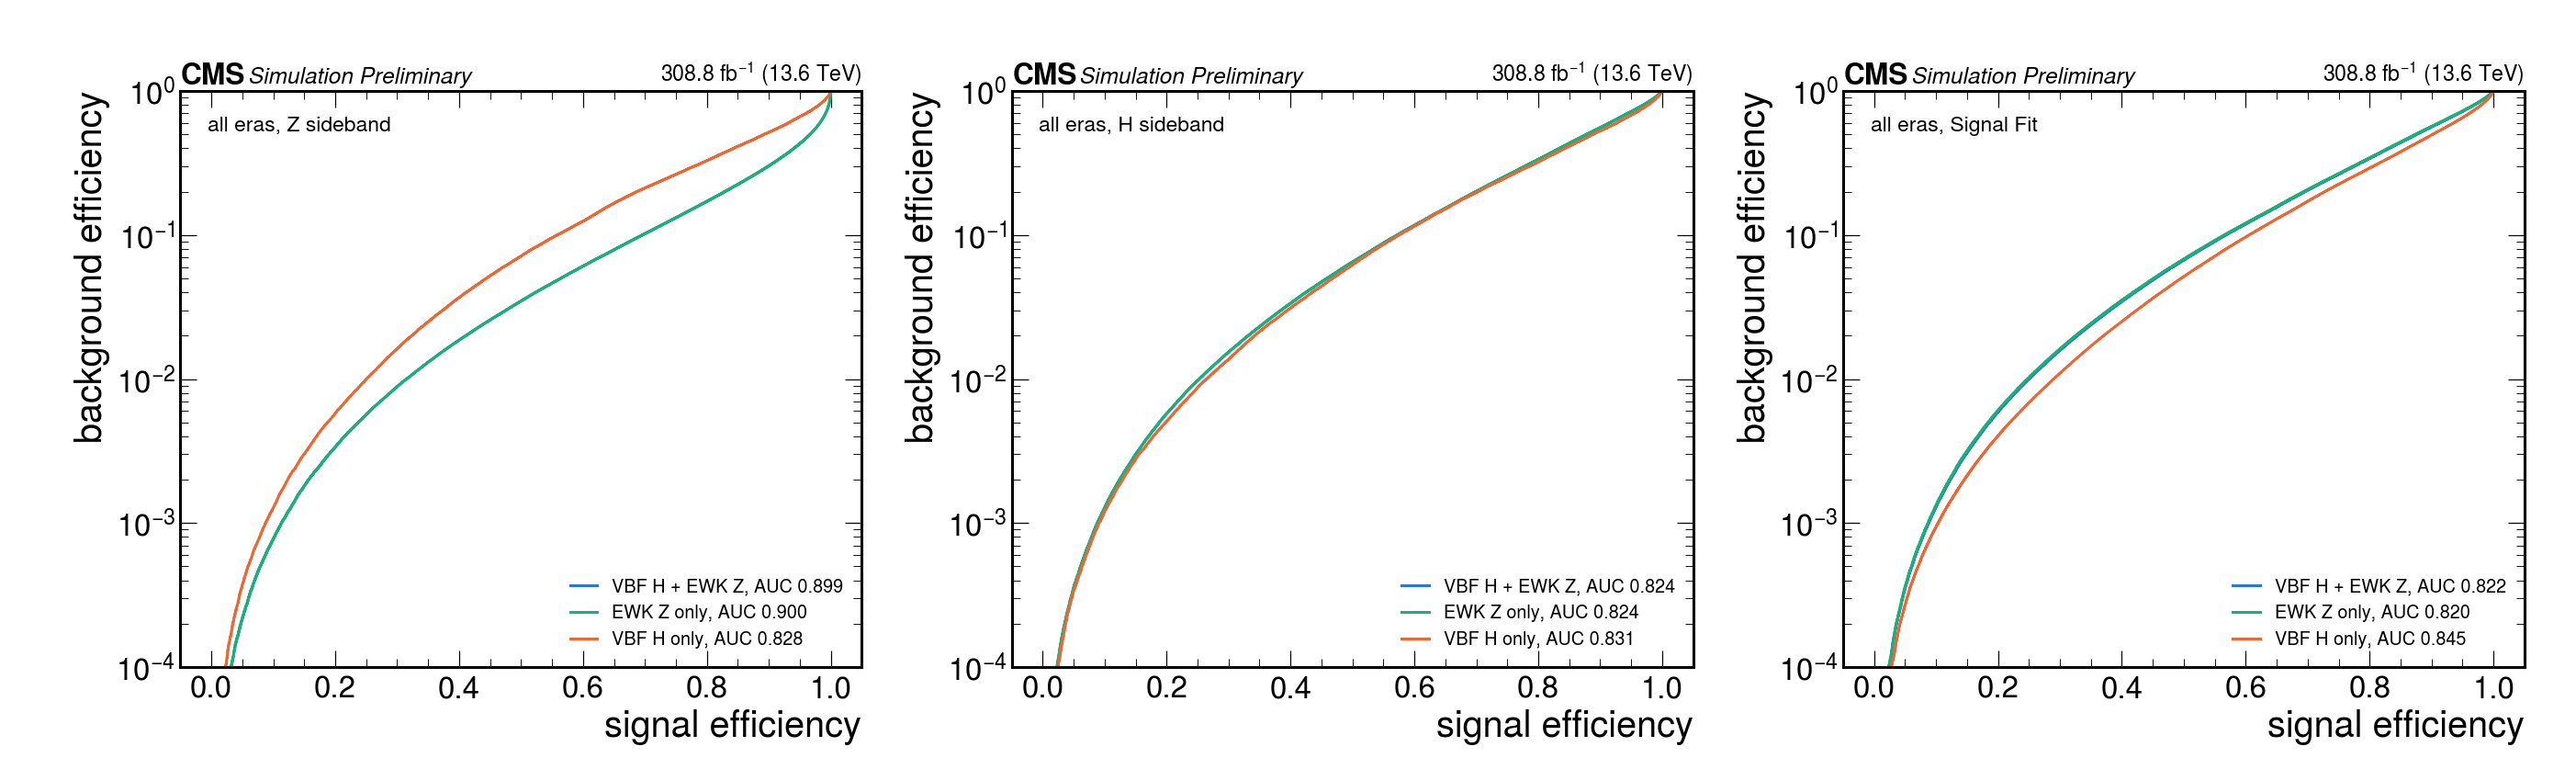
\includegraphics[width=0.49\textwidth]{figures/vbfsel_roc.png}\hfill
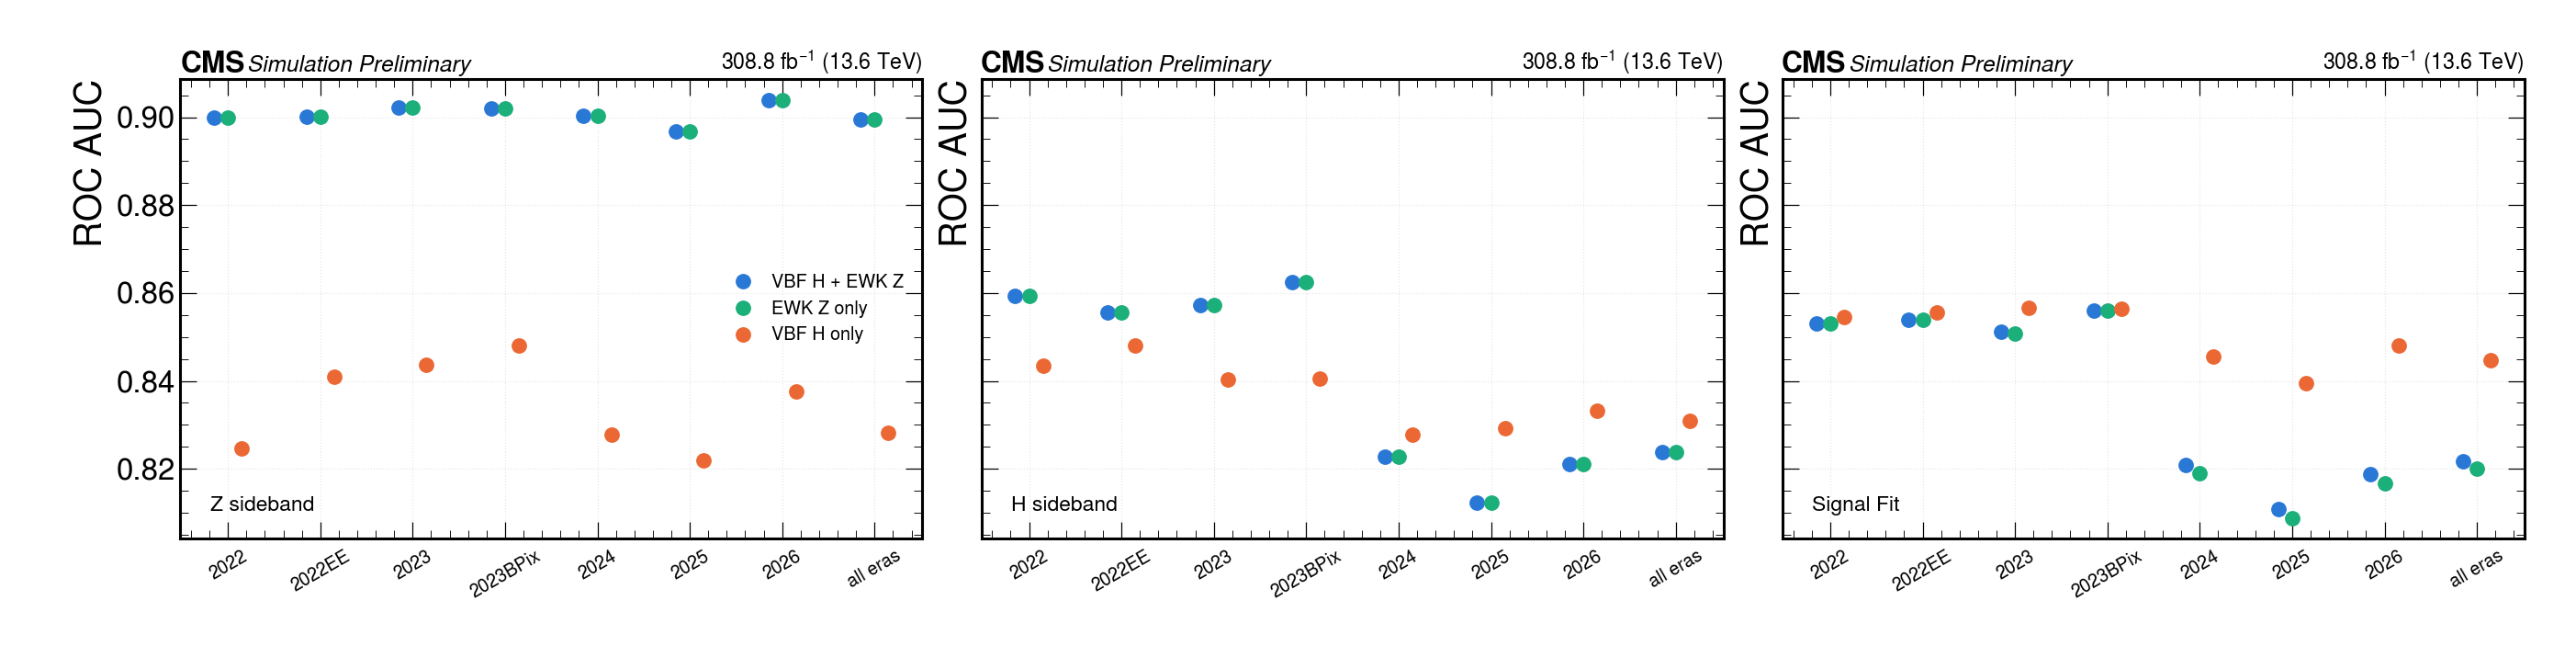
\includegraphics[width=0.49\textwidth]{figures/vbfsel_auc.png}
\caption{VBF selector (\codec{inclusive_regions}): ROC curves per region, all eras
(left), and AUC per era and region (right).
\weblink{studies/vbf_selector/inclusive_regions/}{All figures}; the same set for
\weblink{studies/vbf_selector/sidebands_only/}{sidebands\_only}.}
\end{figure}

\begin{figure}[H]\centering
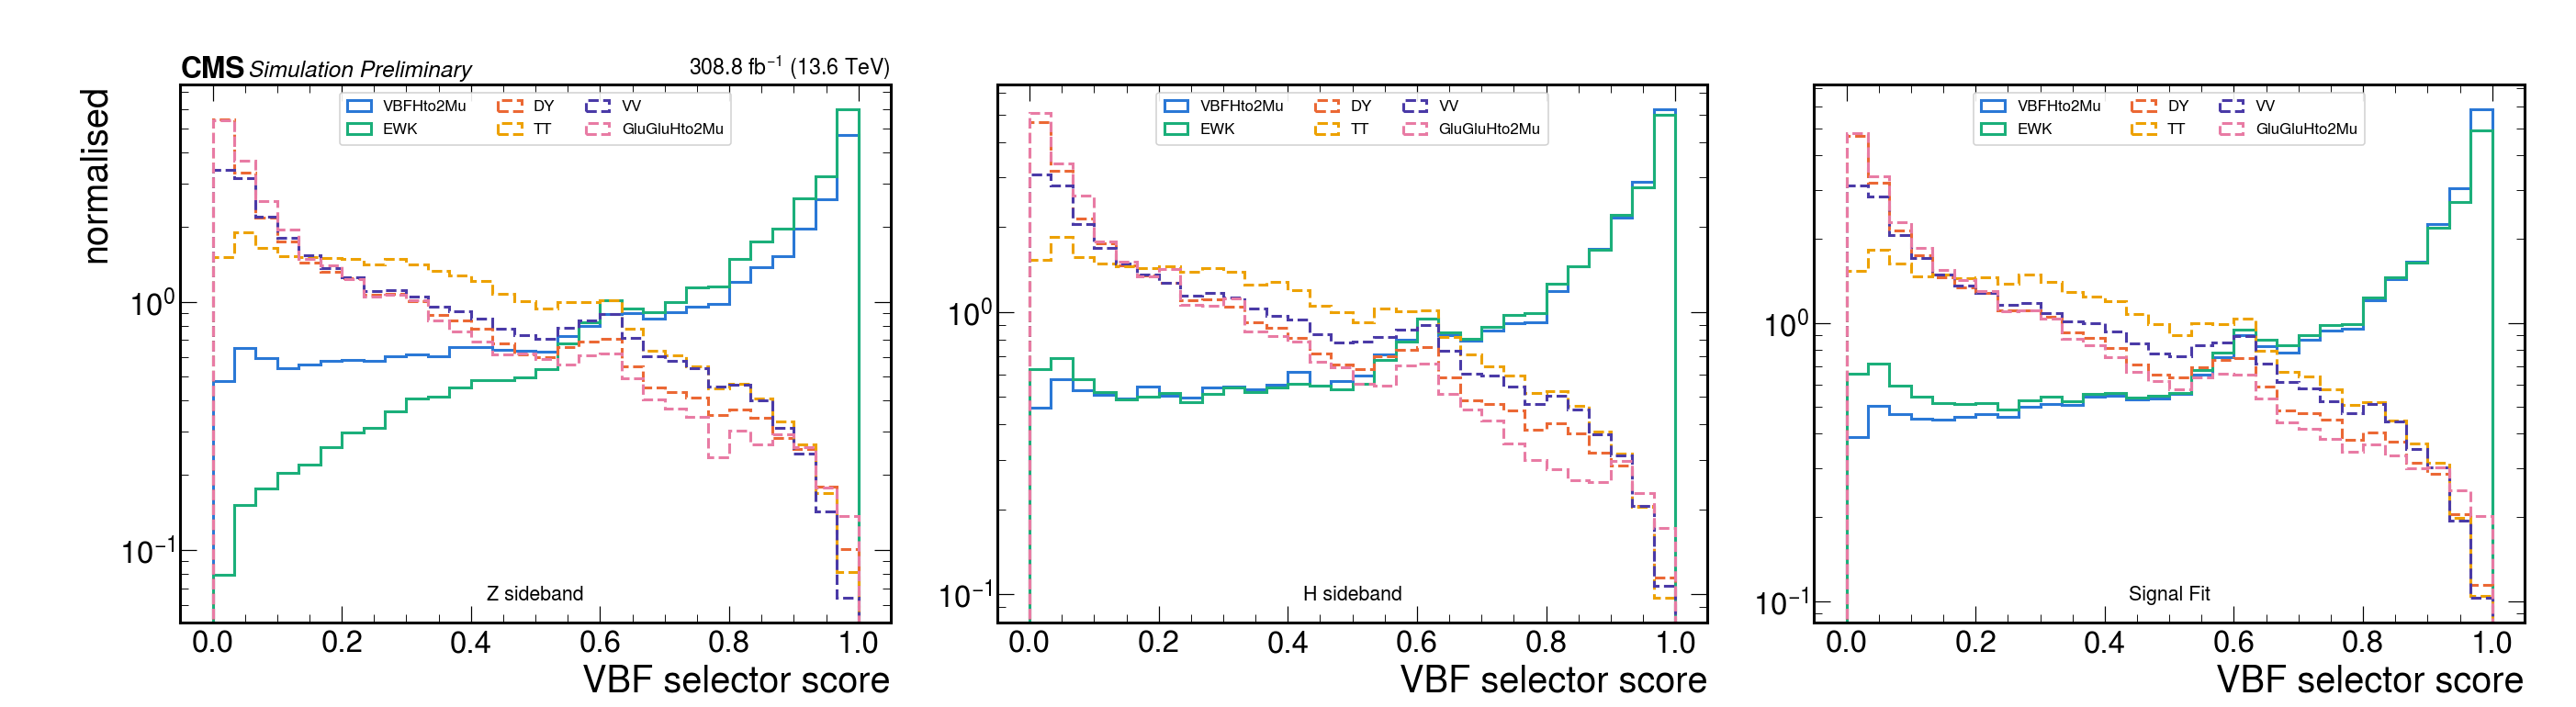
\includegraphics[width=0.75\textwidth]{figures/vbfsel_scores.png}
\caption{Score distributions of signal and background, all eras.}
\end{figure}

\paragraph{SHAP.}
\begin{itemize}
  \item Method: \code{shap.Explainer} on the fold-0 model, using events of the
  held-out fold, half signal and half background.
  \item In every era and region, and for both models, the five leading inputs
  are \code{leadingjet_pt}, \code{leadingjet_eta}, \code{subleadingjet_pt},
  \code{subleadingjet_eta} and \code{pt_mumu}.
  \item In the SR the first one is \code{leadingjet_eta}.
\end{itemize}
The selector is therefore essentially a classifier of the tag-jet kinematics.

\begin{figure}[H]\centering
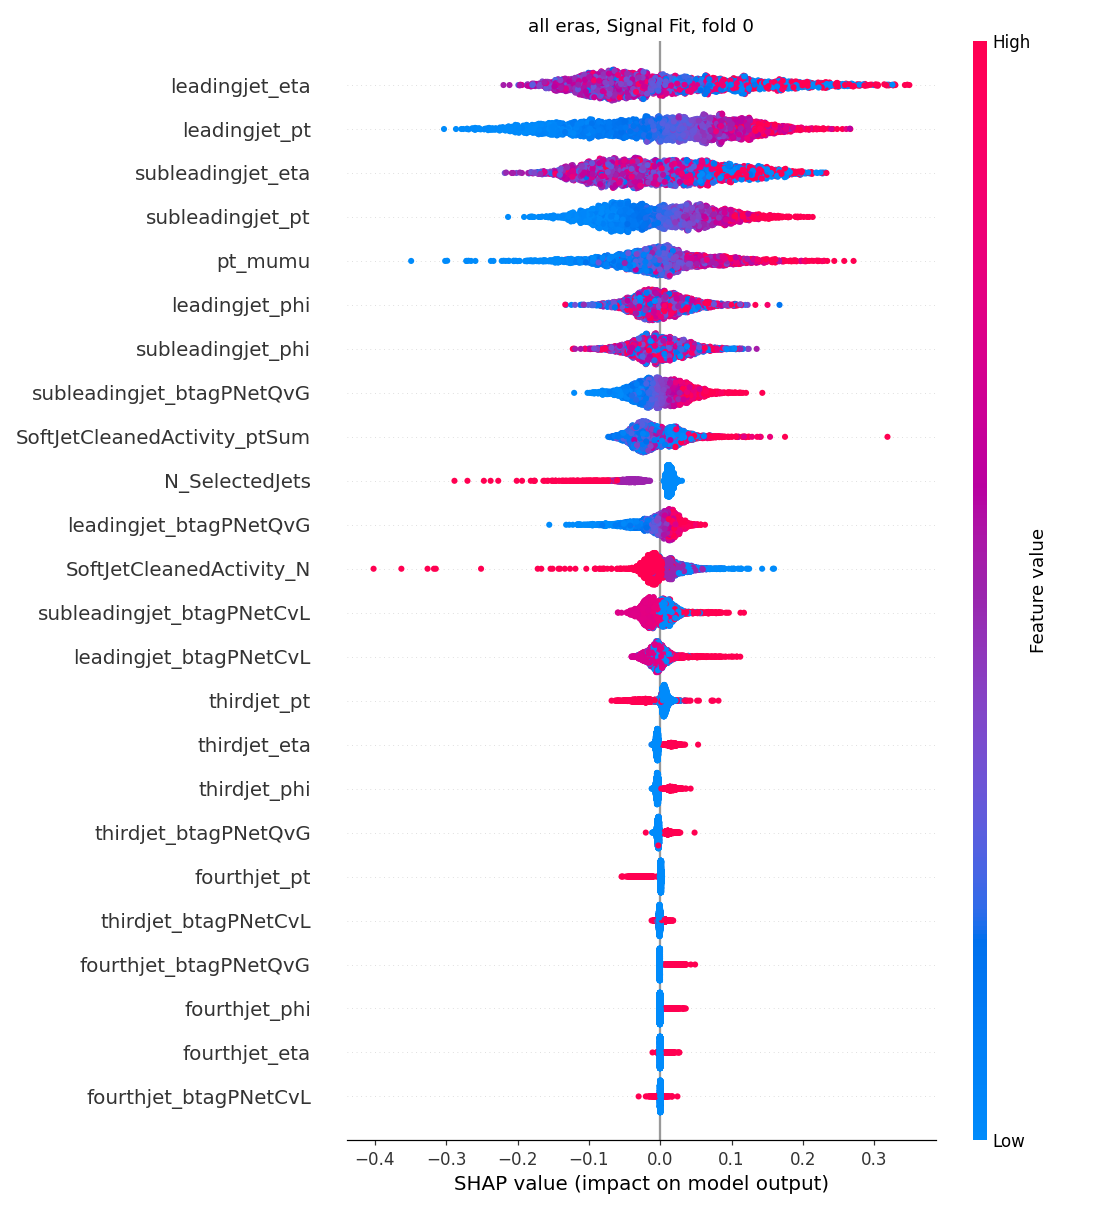
\includegraphics[width=0.7\textwidth]{figures/vbfsel_shap_sr.png}
\caption{SHAP beeswarm in the SR, all eras.
\weblink{studies/vbf_selector/inclusive_regions/shap/}{All eras and regions}.}
\end{figure}

\subsection{Results: selector-defined VBF category (counting)}
\begin{itemize}
  \item Scan of the score threshold in the SR, thresholds 0--0.99 in steps of
  0.01 and then 0.99--1 in steps of 0.001.
  \item $S$ = VBF~H + ggH; $B$ = DY + EWK + $t\bar t$ + VV, with signed
  weights.
  \item The Asimov counting significances of the VBF and ggF categories are
  added in quadrature.
  \item No DNN and no systematics.
\end{itemize}

\begin{table}[H]\centering\small
\begin{tabular}{lccccccccc}
\toprule
category & cut & $\epsilon_\text{VBF H}$ & $\epsilon_\text{ggH}$ & $\epsilon_\text{EWK}$ & bkg rej. & $S_\text{VBF}$ & $B_\text{VBF}$ & $Z_\text{VBF}$ & $Z$ comb. \\
\midrule
selector & 0.96 & 0.219 & 0.008 & 0.184 & 0.9944 & 20.4 & 932 & 0.667 & \textbf{1.105} \\
cut-based & -- & 0.672 & 0.197 & 0.544 & 0.8543 & 113.4 & 24150 & 0.729 & 1.014 \\
\bottomrule
\end{tabular}
\caption{All eras. $Z_\text{ggF}$: 0.882 (selector) and 0.704 (cut-based).}
\end{table}

\begin{table}[H]\centering\small
\begin{tabular}{lccccccc}
\toprule
& 2022 & 2022EE & 2023 & 2023BPix & 2024 & 2025 & 2026 \\
\midrule
best cut & 0.97 & 0.97 & 0.97 & 0.95 & 0.97 & 0.96 & 0.96 \\
$Z$ comb., selector & 0.160 & 0.271 & 0.224 & 0.161 & 0.673 & 0.701 & 0.337 \\
$Z$ comb., cut-based & 0.136 & 0.247 & 0.198 & 0.145 & 0.616 & 0.652 & 0.298 \\
gain & +18\% & +10\% & +13\% & +11\% & +9\% & +8\% & +13\% \\
\bottomrule
\end{tabular}
\caption{Per era.}
\end{table}

The gain comes from the ggF category, which keeps the ggH events that the
cut-based VBF category takes away. The tight VBF category alone is worse than
the cut-based one. This has to be repeated with the DNN fit.

\begin{figure}[H]\centering
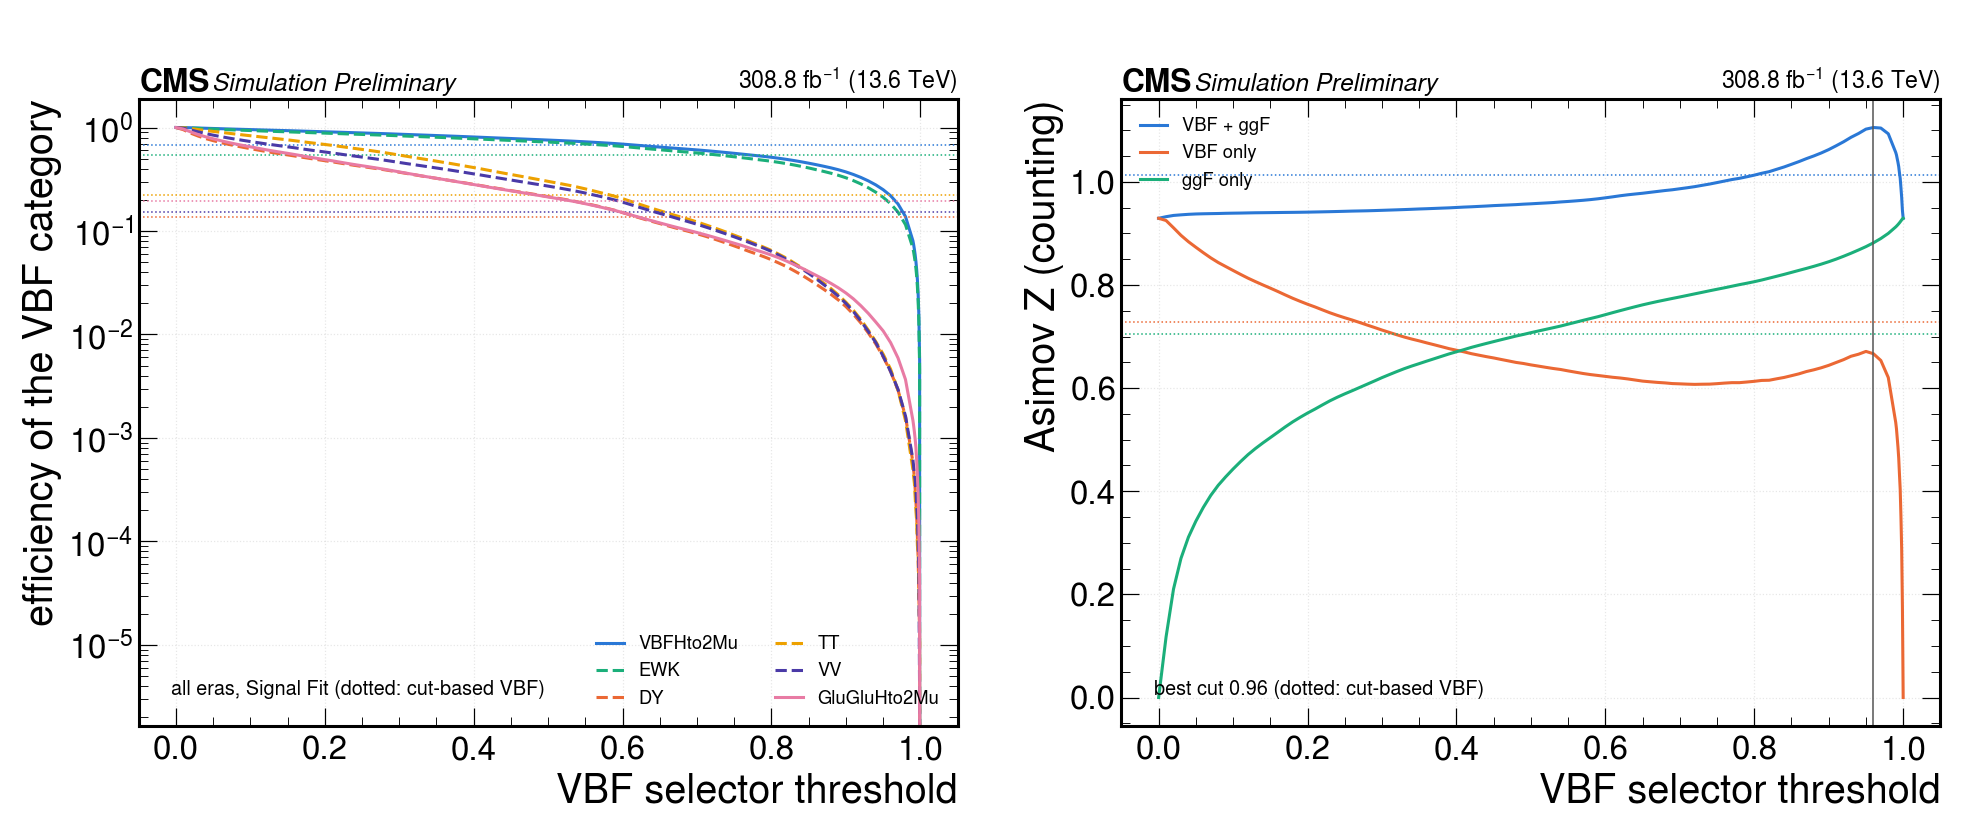
\includegraphics[width=0.8\textwidth]{figures/vbfsel_cutscan.png}
\caption{Cut scan on the selector score in the SR, all eras.}
\end{figure}

\subsection{Results: EWK~Z fit in the sidebands}

\paragraph{Fit set-up} (\code{studies/vbf_selector/fit_ewkz_systematics.py}):
\begin{itemize}
  \item one channel per era and sideband (\code{zsb_<era>} and \code{hsb_<era>}),
  using the score in \code{baseline_ge2J};
  \item POI $r_\text{EWK}$;
  \item processes EWK, VBFH, ggH, TT, ST, TW, VV, VVV, TTX, VH, ttH and DY;
  \item lnN on luminosity and on the cross sections per source;
  \item \code{autoMCStats}.
\end{itemize}
DY models:
\begin{itemize}
  \item \code{hard-pu} (main): DY Hard and DY PU, each with a free rateParam
  per channel in [0.05, 10];
  \item \code{hard-pu-lnn}: as \code{hard-pu} with lnN constraints;
  \item \code{single}: one free DY;
  \item \code{hard-pu1-pu2}: three components, diagnostic only.
\end{itemize}

\paragraph{Quick fit} (29~September, training tuples, no systematics, one free
DY per channel): ZSB $0.918\pm0.038$, HSB $2.08\pm0.15$, combined
$0.997\pm0.036$. The eras range from 0.43 to 1.52. This fit is superseded.

\paragraph{Campaign fit} (30~September, Central templates, no shape
systematics):

\begin{table}[H]\centering\small
\begin{tabular}{lcccc}
\toprule
era & Z sideband & H sideband & Z + H & obs.\,/\,exp.\ significance \\
\midrule
all & 1.020 & 1.699 & \textbf{1.051}$^{+0.033}_{-0.032}$ & 45.5 / 41.9 \\
2022 & 0.596 & 1.626 & $0.616\pm0.124$ & 5.1 / 8.1 \\
2022EE & 0.836 & 1.313 & $0.846\pm0.069$ & 12.7 / 15.2 \\
2023 & 0.673 & 0.443 & $0.669\pm0.097$ & 6.9 / 10.2 \\
2023BPix & 1.023 & 1.057 & $1.024\pm0.140$ & 7.4 / 7.2 \\
2024 & 1.241 & 1.775 & $1.268\pm0.055$ & 32.5 / 25.9 \\
2025 & 1.155 & 2.055 & $1.230^{+0.086}_{-0.082}$ & 26.6 / 23.4 \\
2026 & 1.065 & 1.405 & $1.094^{+0.136}_{-0.130}$ & 8.8 / 9.3 \\
\bottomrule
\end{tabular}
\caption{EWK~Z signal strength on data, \codec{hard-pu}
(\codec{combine/results_vbf_selector_ewkz_syst/}\linebreak\codec{no_shape_systematics/}).}
\end{table}

\begin{itemize}
  \item Combined fit: statistical error $\pm0.013$; expected significance 44.3
  with toysFreq.
  \item Separate sidebands: ZSB 44.0/41.1 and HSB 12.6/8.2 (observed/expected).
  \item Other DY models, all eras, Z+H:
  \begin{itemize}
    \item \code{hard-pu-lnn}: $1.118\pm0.028$;
    \item \code{single}: $0.804\pm0.032$, which fails in 2025 (0.28).
  \end{itemize}
\end{itemize}

\begin{figure}[H]\centering
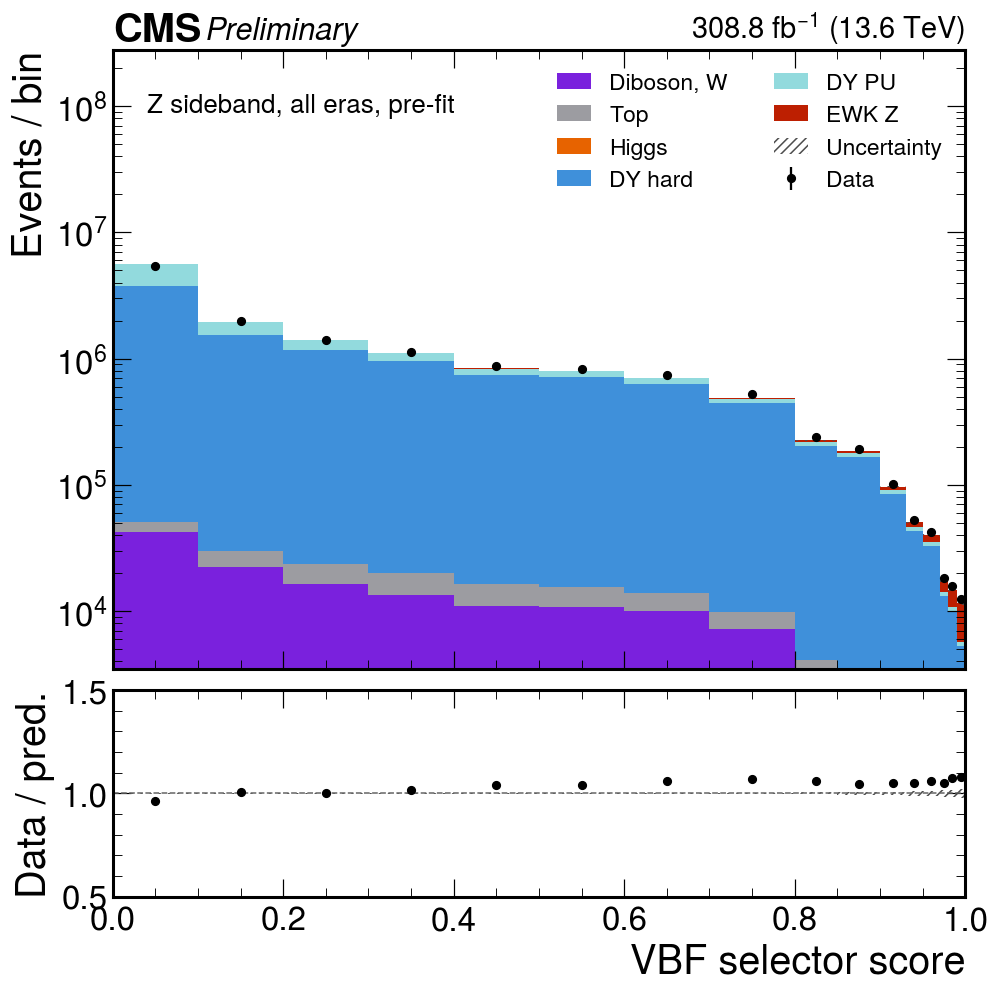
\includegraphics[width=0.32\textwidth]{figures/vbfsel_prefit_zsb.png}\hfill
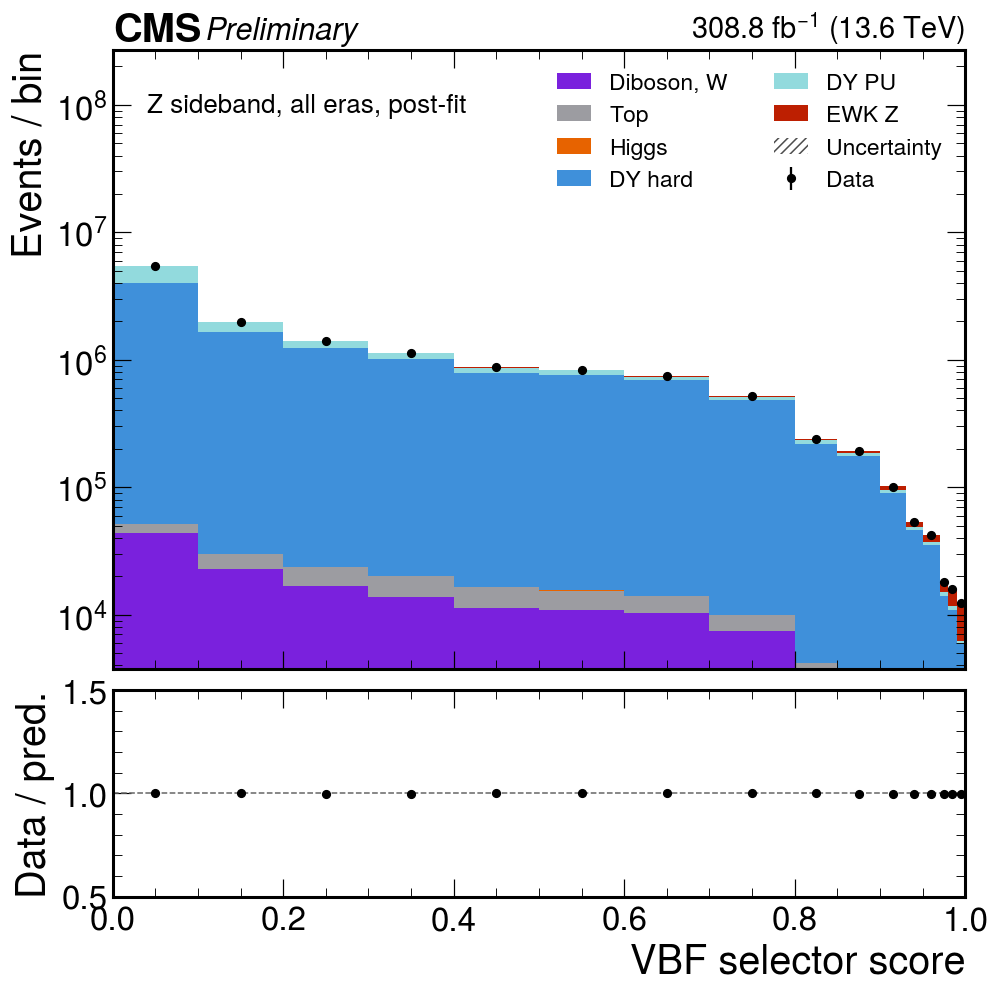
\includegraphics[width=0.32\textwidth]{figures/vbfsel_postfit_zsb.png}\hfill
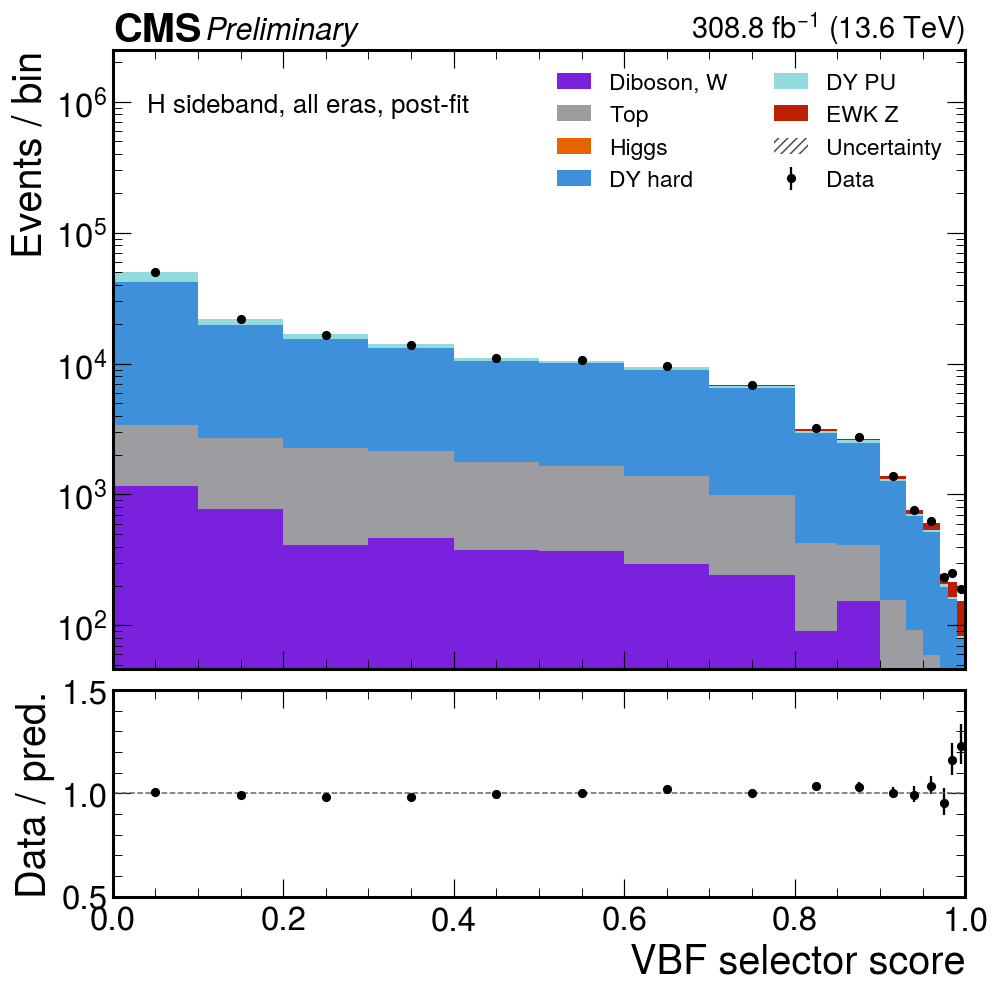
\includegraphics[width=0.32\textwidth]{figures/vbfsel_postfit_hsb.png}
\caption{EWK~Z fit, \codec{hard-pu}: pre-fit in the Z sideband, and post-fit in the
Z and H sidebands.
\weblink{studies/vbf_selector/ewkz_fit/no_shape_systematics/}{All models and eras}.}
\end{figure}

\paragraph{Not yet a measurement.}
\begin{itemize}
  \item The eras range from 0.62 to 1.27, and the two sidebands disagree
  (Z 1.02, H 1.70).
  \item Pre-fit data/DY in the ZSB rises from 0.96 at low score to about 1.07
  above 0.7. Era by era, the ZSB data/MC goes from 1.05 down to 0.90 in 2022--22EE,
  is flat in 2023--23BPix, is $+5\%$ in 2024 and $+10$--$20\%$ in 2025--26.
  \item The Hard/PU split of DY reduces the sideband disagreement from
  2.1/0.92 to 1.7/1.02, but the DY shape is still mismodelled. In the data fit
  the ZSB MC-statistics parameters are pulled by up to $7\sigma$ (2025).
  \item Shape systematics are needed before $r_\text{EWK}$ can be used.
\end{itemize}

%=====================================================================
\section{Comparison of the two networks}
%=====================================================================

\begin{table}[H]\centering\small
\begin{tabularx}{\textwidth}{lYY}
\toprule
& analysis DNN & VBF selector \\
\midrule
question & is it $H\to\mu\mu$? & is it a VBF topology? \\
signal & VBF~H + ggH & VBF~H + EWK~Z$jj$ \\
training region & cut-based VBF category, SR & \code{baseline_ge2J}, ZSB + HSB + SR \\
dimuon mass & input (\code{m_mumu}) & not used \\
inputs & 32: muons, dimuon, angles, tag jets, soft activity, era & 24: four leading jets, $p_T^{\mu\mu}$, soft activity \\
network & $4\times86$, ReLU, no regularisation & $4\times100 + 2\times50$, BatchNorm + dropout 0.1 \\
training eras & 2022--2025 (with \code{era_code}) & 2022--2026 (no era input) \\
weights & absolute value & signed \\
typical AUC & 0.89--0.91 (SR, VBF) & 0.90 (ZSB), 0.82 (HSB, SR) \\
use & fit variable of $H\to\mu\mu$ & EWK~Z fit; alternative VBF category \\
status & production; retraining ready & payload \code{VBFSel} installed; systematic fit pending \\
\bottomrule
\end{tabularx}
\end{table}

%=====================================================================
\section{Fit plan: what exists and what is missing}\label{sec:plan}
%=====================================================================

The state below is as of 7~October~2026, 15:00.
\begin{itemize}
  \item \textbf{Order.} Everything is done first for the inclusive VBF
  category. Only after the inclusive chain is complete and validated is the
  CC/CF/FF split run.
  \item \textbf{Templates.} The DNN templates with full systematics are
  \code{dnn_vbf_eta_regions_syst} (\code{incl} sub-directory for the inclusive
  fits; CC, CF and FF for the split). They replace \code{dnn_vbf_weighted}.
  \item \textbf{Automation.} The chain
  \code{combine/results_fit_matrix/logs/chain_20261007d.sh} runs the remaining
  steps: rebuild of the hadds, merge, validation of the shifted templates, then
  the fits only if no critical flag.
\end{itemize}

\subsection{Templates}

\begin{table}[H]\centering\small
\begin{tabularx}{\textwidth}{>{\raggedright}p{0.25\textwidth}>{\raggedright}p{0.2\textwidth}>{\raggedright}p{0.1\textwidth}Y}
\toprule
campaign & content & state & notes \\
\midrule
\code{dnn_vbf_weighted} & DNN, VBF, all syst. & \inval & score not re-evaluated for JES/JER/muon scale; to be deleted \\
\code{dnn_vbf_eta_regions} & DNN, incl/CC/CF/FF, Central & \done & used for the CC/CF/FF study without systematics \\
\code{dnn_vbf_eta_regions_syst} & DNN, incl/CC/CF/FF, all syst., Hard/PU & \prog & all seven eras merged on 7~October; broken hadds found (ScaRe DY M-50 2024--25, QCD scales DY 2025, Muon 2022/2025, JER up$=$down 2022--22EE), being rebuilt and validated \\
\code{dnn_vbf} & DNN, VBF, five regions, all syst. & \prog & for plots; jobs running \\
\code{vbf_selector_ewkz} & selector + 24 inputs, ZSB/HSB, all syst. & \prog & merge-syst only for 2022; VBF~H powheg+Herwig 2024--26 and a few datasets added; 2024 preliminary merge in use \\
\code{vbf_selector_ewkz_eta} & selector, VBF incl/CC/CF/FF, all syst. & \prog & histogram jobs running; not merged \\
\code{vbf_eta_regions_syst} & all variables, incl/CC/CF/FF, all syst. & \prog & data/MC with systematic bands per $\eta$ category \\
\bottomrule
\end{tabularx}
\caption{Template campaigns.}
\end{table}

Known template issues, which are expected and not bugs:
\begin{itemize}
  \item JEReta2pt0 and JEReta3pt0 ($|\eta|>2.5$, $p_T<50$~GeV) have no effect,
  because those jets are removed by the horn veto.
  \item The QCD scales of EWK~Z are flat, because it is an LO electroweak process.
  \item 2026 has no muon scale factors and therefore no muon-efficiency
  uncertainty. A prescription is still to be decided (2025 scale factors or a
  flat value).
  \item 2026 has no luminosity nuisance of its own and uses \code{lumi_2025}.
\end{itemize}

\subsection{$H\to\mu\mu$ fits with the DNN}

\begin{longtable}{>{\raggedright}p{0.035\textwidth}>{\raggedright}p{0.34\textwidth}>{\raggedright}p{0.14\textwidth}>{\raggedright}p{0.1\textwidth}>{\raggedright\arraybackslash}p{0.22\textwidth}}
\toprule
& fit & systematics & state & result / output \\
\midrule
\endhead
\multicolumn{5}{l}{\emph{Inclusive VBF category}} \\
D1 & SR + HSB and SR only, 4 DY models, pre-fit and toysFreq, each era and all eras (fit matrix) & full, old templates & \inval & 2.102 (\code{lnn}, toysFreq); \code{results_fit_matrix/dnn_sr}, \code{dnn_sr_hsb} \\
D2 & as D1, 6 eras (2022--25), one-line \code{--toysFreq} & full, old templates & \inval & 1.998; superseded \\
D3 & SR + HSB, DY scale V shape-only & full, old templates & \inval & 2.172 pre-fit (30~Sept.) \\
D4 & EWK~Z normalisation test ($\pm0.5\%$, 10\%, 30\%, free) & full, old templates & \done & 2.14 $\to$ 1.63 \\
D5 & data fit of ZSB + HSB with the SR masked (post-fit sidebands) & full, old templates & \done & \code{dnn_sr_hsb_zsb} \\
D6 & SR + HSB incl, Central cards (stat + lumi + MC stat), pre-fit and toysFreq & none & \done & 2.350 / 2.366 \\
D7 & SR + HSB and SR only, 4 DY models, significance, limits, impacts, scans (\code{results_7eras_v2/}: \code{base}, \code{SRonly}, \code{DYscaleShapeOnly}) & full, \textbf{new templates} & \miss & runs in the chain after validation \\
D8 & fit matrix v2: each era and all eras, pre-fit and toysFreq, impacts everywhere, post-fit HSB (\code{results_fit_matrix_v2}) & full, new templates & \miss & runs in the chain after D7 \\
D9 & stat-only and per-group breakdown on D7/D8 & -- & \miss & from \code{fit_suite.py} \\
\midrule
\multicolumn{5}{l}{\emph{VBF split CC/CF/FF} (only after the inclusive fits are validated)} \\
D10 & CC/CF/FF, Central cards, 6 and 7 eras, pre-fit and toysFreq (SR masked) & none & \done & +1.8\% (2.366 $\to$ 2.410) \\
D11 & CC/CF/FF with free DY per era and $\eta$ category & none & \done & +1.9\% \\
D12 & CC/CF/FF, 4 DY models, Hard/PU split, all eras (\code{results_7eras_v2/CCCFFF}) & full, new templates & \miss & in the chain; checks that the +1.8\% survives systematics \\
D13 & CC/CF/FF fit matrix per era, impacts & full, new templates & \miss & not yet scheduled \\
D14 & FF data/MC at high score: dedicated DY treatment or FF nuisance & -- & \miss & needed if FF is kept \\
\midrule
\multicolumn{5}{l}{\emph{Later}} \\
D15 & $H\to\mu\mu$ card with the EWK~Z constraint from the selector fit (V3) & full & \miss & after V3 \\
D16 & retrained DNN (7 eras; with and without \code{m_mumu}), same campaign and card as D7 & full & \miss & training not started \\
D17 & DNN fit in the selector-defined VBF category & full & \miss & needs a new campaign \\
\bottomrule
\caption{Fits with the analysis DNN. ``Old templates'' $=$ \codec{dnn_vbf_weighted}
(jet/muon systematics invalid); ``new templates'' $=$ \codec{dnn_vbf_eta_regions_syst}.}
\end{longtable}

\subsection{EWK~Z fits with the VBF selector}

\begin{longtable}{>{\raggedright}p{0.035\textwidth}>{\raggedright}p{0.34\textwidth}>{\raggedright}p{0.14\textwidth}>{\raggedright}p{0.1\textwidth}>{\raggedright\arraybackslash}p{0.22\textwidth}}
\toprule
& fit & systematics & state & result / output \\
\midrule
\endhead
\multicolumn{5}{l}{\emph{\code{baseline_ge2J}, no $\eta$ split}} \\
V0 & quick fit on the training tuples, one DY per channel & lumi + flat lnN & \done & 0.997; superseded (\code{combine/archive/}) \\
V1 & campaign templates, Central, ZSB, HSB and Z+H, each era and all eras, DY models \code{single}, \code{hard-pu}, \code{hard-pu-lnn}, \code{hard-pu1-pu2} & lumi + xsec + MC stat & \done & $1.051\pm0.033$ (\code{hard-pu}) \\
V2 & fit matrix of V1: pre-fit and toysFreq Asimov, data, pulls, impacts & as V1 & \done & expected 41.9 / 44.3, observed 45.5 \\
V2b & 2024 only, preliminary merge, all shape systematics, \code{single}/\code{hard-pu}/\code{hard-pu-lnn} & full & \prog & \code{combine/results_vbf_selector_ewkz_2024_prelim}; a check before the full set \\
V3 & all eras, all shape systematics, three DY models (\code{results_vbf_selector_ewkz_syst/systematics}) & full & \miss & in the chain; needs merge-syst for every era \\
V4 & fit matrix of V3 (\code{results_fit_matrix_v2/vbfsel_systematics}) & full & \miss & in the chain after V3 \\
V5 & pre-fit data/MC of the score and of the 24 inputs with the systematic band & full & \miss & after the merge \\
\midrule
\multicolumn{5}{l}{\emph{VBF category split CC/CF/FF} (only after V3--V5)} \\
V6 & selector templates in the VBF category per $\eta$ class (\code{vbf_selector_ewkz_eta}) & full & \prog & histograms only \\
V7 & EWK~Z fit per $\eta$ class (\code{r} common or per class), with the DY Hard/PU split & full & \miss & card builder to be extended; tests whether the FF excess is EWK~Z or DY \\
V8 & performance and data/MC of the selector per $\eta$ class & -- & \miss & \\
\midrule
\multicolumn{5}{l}{\emph{Selector as a category}} \\
V9 & selector-defined VBF category: cut optimisation with the DNN fit, full systematics & full & \miss & counting gives +9\%, from the ggF side \\
\bottomrule
\caption{Fits with the VBF selector.}
\end{longtable}

\subsection{Order of execution}
\begin{enumerate}
  \item \textbf{Templates, inclusive.} Rebuild the broken hadds of
  \code{dnn_vbf_eta_regions_syst} and \code{vbf_selector_ewkz}, merge-syst for
  every era, and \code{tools/validate_variations.py} with no critical flag.
  \item \textbf{DNN, inclusive, full systematics:} D7 and D8 (with D9). This
  gives the new reference significance, which replaces 2.102.
  \item \textbf{EWK~Z, inclusive, full systematics:} V3, V4 and V5. Check
  whether the two sidebands and the eras become compatible once the shape
  systematics are included.
  \item \textbf{Checkpoint:} report the inclusive results before any split.
  \item \textbf{CC/CF/FF:} D12 and D13 for the DNN, V6--V8 for the selector, and
  D14 if FF is kept.
  \item \textbf{Combination:} D15 (EWK~Z constraint in the $H\to\mu\mu$ card).
  Then D16 (retrained DNN) and D17/V9 (selector category).
\end{enumerate}

\subsection{Open decisions}
\begin{itemize}
  \item 2026 muon scale factors (2025 values or a flat uncertainty) and the
  2026 luminosity nuisance.
  \item Which DY model is the reference for the $H\to\mu\mu$ fit (\code{lnn} today)
  and for the EWK~Z fit (\code{hard-pu}).
  \item Whether to keep FF, given its data/MC at high DNN score.
  \item Whether to remove \code{m_mumu} from the DNN.
\end{itemize}

%=====================================================================
\section*{References in the repository}
%=====================================================================
\begin{itemize}
  \item DNN:
  \begin{itemize}
    \item \code{common/updated_DNN_configs/config.toml};
    \item \code{common/dnn_application.py};
    \item \code{studies/dnn/README.md}, \code{studies/dnn/retraining/README.md};
    \item \code{config/campaigns/dnn_vbf*.sh}.
  \end{itemize}
  \item Fits:
  \begin{itemize}
    \item \code{combine/README.md}, \code{combine/RESULTS.md},
    \code{combine/COMPARISON_20261006.md};
    \item \code{combine/results_fit_matrix/SUMMARY.md},
    \code{combine/results_fit_matrix/VALIDATION_20261007.md};
    \item \code{docs/status.md}.
  \end{itemize}
  \item VBF selector:
  \begin{itemize}
    \item \texttt{studies/vbf\_selector/\{README,RECAP,RESULTS,STATUS\}.md};
    \item \code{common/vbfsel_configs/config.toml};
    \item \code{config/campaigns/vbf_selector_ewkz*.sh};
    \item \code{docs/ewkz_fit_motivation.md}.
  \end{itemize}
  \item Plots:
  \begin{itemize}
    \item \url{\www/studies/dnn/}, \url{\www/dnn/};
    \item \url{\www/studies/vbf_selector/};
    \item \url{\www/fits/}.
  \end{itemize}
\end{itemize}

\end{document}
